\chapter{Simulaciones Monte Carlo}\label{cap:simulaciones}

En este capítulo se describe como fueron simulados los procesos del modelo de
SUSY (\cref{sec:sig_samples}) y los procesos del SM (\cref{sec:bkg_samples}) que
dan lugar al estado final de interés. Todas las muestras fueron simuladas
utilizando generadores Monte Carlo a $\sqrt{s}=8\tev$. A continuación se simuló
el pasaje por el detector ATLAS para luego ser reconstruidas con los mismos
algoritmos que los datos observados.

%% La mayoría de los fondos MC fueron utilizados para comparaciones y cross checks.
%% La estimación de los fondos  en las regiones de señal se estimó cuando fue posible de los
%% propios datos observados.

%% Todas las muestras fueron pasadas a través de la simulación completa basada en Geant4\cite{Geant4,AtlasSim} o rápida
%% ATLFAST-II\cite{Richter-Was:683751} del detector ATLAS, y reconstruidas con los mismos algoritmos
%% que se utilizaron para los datos.

%% un repesado evento a eventos es aplicado a todas las muestras MC para modelar las condiciones
%% realistas de las muestra de datos bajo estudio, matcheando la distribución del numero de interaccionas
%% por cruze de bunchs (pile-up) de las muestras simuladas a la observada en datos.



\section{Simulación de la se\~nal}\label{sec:sig_samples}

\subsection{Generación de eventos}

La conexión entre la teoría/fenomenología de SUSY (o cualquier otra teoría de
nueva física), y las observaciones experimentales en el detector de un
colisionador se realiza por medio de un \emph{generador de eventos}. Dada una
teoría de nueva física, que en general predice la existencia de nuevas
partículas y/o interacciones, el generador de eventos permite calcular cómo esa
teoría se manifiesta en el experimento\cite{Baer:2009tk}.

El procedimiento, una vez que se selecciona un modelo particular de SUSY,
requiere de varios pasos que se encuentran esquematizados en la
\cref{fig:mc_sketch}. En primer lugar es necesario calcular el espectro de masas
de las partículas supersimétricas, y sus acoplamientos. A partir de esto se
calculan los anchos y tazas de decaimiento de todas estas partículas. Y por
último se utiliza el generador, que toma como entrada las masas y decaimientos
calculados previamente, y genera los eventos de SUSY. Para las distintas etapas
suelen utilizarse herramientas diferentes, por lo que es fundamental contar con
un forma estandarizada de intercambio de información entre ellas. Con este
objetivo se creo un tipo de archivo llamado SLHA (SUSY Les Houches
Accord)\cite{SLHA} que permite organizar toda la información de un cierto modelo
de supersimetría (parámetros, masas, decaimientos) en un solo lugar y de forma
que sea fácil de compartir entre los físicos y también los distintos software.

\begin{figure}[h]
  \centering
  \scalebox{0.8}{\begin{tikzpicture}[node distance=1.5cm, auto,]

    \node[rec] (susy) {\sc Modelo SUSY};
    \node[rec, right=of susy] (masses) {\sc Espectro de Masas};
    \node[rec, right=of masses] (decays) {\small \sc Decaimientos};
    \node[rec, right=of decays] (gen) {\sc Generador de Eventos};
    \node[rec, right=of gen] (atlas) {\sc Simulación Detector};

    \draw[arr] (1.7,0) -- (2.7,0);
    \draw[arr] (6.2,0) -- (7.2,0);
    \draw[arr] (10.8,0) -- (11.7,0);
    \draw[arr] (15.1,0) -- (16.1,0);

\end{tikzpicture}
}
  \caption{Etapas de la generación de eventos de un modelo de SUSY.}
  \label{fig:mc_sketch}
\end{figure}

%% Para interfacear dos o mas calculos, el procedimiento general requiere que
%% el usuario prepare los parametros del modelo ,
%% junto con un conjunto de parametros
%% del SM (que seran usados como las
%% condiciones de contorno a escala de baja energia para el calculo del espectro),
%% en un archivo de texto , siguiendo el acuerdo SLHA.

%% Luego se corre un generador de espectro con este archivo como entrada para obtener
%% las masas de las particulas SUSY y los acoplamientos a la escala electrodebil.
%% El espectro resultante es guardado, junto con una copia de los parametros de entrada)
%% en un nuevo archivo.

%% El siguiente paso es utilizar un programa que genere los modos de decaimiento y sus anchos
%% para las particulas seleccionadas, que se guarda en un tercer archivo, junto con la copia
%% de los parametros de entrada y el espectro de masas.

%% Y por ultimo, se utiliza un generador de eventos (completo o a nivel partonico) que
%% genera los eventos a partir de la informacion de este archivo.


\subsubsection{Espectro de masas y decaimientos}

Los modelos de SUSY que se estudian en un colisionador suelen ser la teoría
efectiva a bajas energías que resultan de una teoría mas general, como teoría de
supercuerdas, o que involucre un mecanismo particular para el rompimiento de
SUSY. Para especificar una teoría efectiva es necesario definir: (1) la simetría
de gauge, (2) los campos que la componen y, (3) el Lagrangiano. Los efectos del
rompimiento de SUSY están codificados en los términos de rompimiento soft del
Lagrangiano. También se debe especificar la escala de energía a la cual la
teoría efectiva y el lagrangiano son válidos. Y como los experimentos testean
física a la escala débil $Q\sim 1 \tev$, mientras que los parámetros del
Lagrangiano son frecuentemente especificados a energías mucho mas altas
($M_\text{GUT}$ o $M_P$), debe usarse el grupo de ecuaciones de renormalización
(RGE) para conectar las dos escalas del modelo.
Una vez que los parámetros del Lagrangiano son conocidos a la escala
electrodébil, pueden identificarse las masas físicas de las partículas,
diagonalizando las matrices de masa correspondientes, y luego, para tener la
precisión suficiente, aplicar las correcciones a ordenes mayores (en general a 1
loop). A partir del modelo también es posible calcular los anchos y tazas de
decaimiento de todas las partículas supersimétricas.

Existe una gran variedad de programas que permiten realizar estos cálculos.
En este trabajo utilizamos el programa
{\susyhit}\cite{Djouadi:2006bz} que combina {\suspect}\cite{Djouadi2007426}
para calcular el espectro de masas, junto
con {\sdecay}\cite{Muhlleitner:2004mka} y {\hdecay}\cite{Djouadi:1997yw}
para calcular los BRs y anchos de decaimiento. Algunos de estos modos de
decaimientos son calculados a NLO en QCD.

%% {\suspect}\note{referencia} corre las RGE a dos loops en el MSSM para determinar
%% los parametros de SUSY a la escala electrodebil en modelos de mSUGRA, GMSB, AMSB
%% y pMSSM. Y aplica luego las correscciones a 1 loop, y algunas correcciones a 2 loops
%% para las masas de los Higgs.

Una vez que el espectro de masas y los decaimientos están calculados estos
pueden usarse como entrada en los generadores de eventos.

%% % SLHA
%% Para facilitar el intercambio de información entre distintos programas de SUSY
%% se propuso una seria de convenciones: SUSY Les Houches Accord (SLHA)\cite{SLHA}.
%% Este acuerdo permite usar la salida de los códigos que calculan el espectro de
%% masa y decaimientos como entrada en los generadores de eventos de una forma
%% consistente y sin ambigüedades.

%% %% En general estos modelos pueden
%% %% ser teorias efectivas
%% La teoria efectiva queda especificada adoptando la simetria de
%% gauge, the (super)field content y el Lagrangiano.
%% {\suspect} runs the 2-loop MSSM RGEs to determine weak scale
%% SUSY parameters in the mSUGRA, GMSB and AMSB models,
%% and in the pMSSM (a more general MSSM model). One-loop
%% sparticle mass corrections are included.
%% Some two loop corrections to Higgs masses are included.


\subsubsection{Generador de eventos}

Los programas descriptos anteriormente permiten pasar de un modelo de SUSY a las
predicciones en la producción de partículas y sus anchos de decaimientos en
estados finales de quarks, leptones, fotones y gluones (y LSP en modelos donde
se conserva paridad-R). Sin embargo los quarks y gluones no pueden medirse
directamente en los detectores. Los detectores pueden medir trazas de partículas
(cuasi)estables cargadas y su momento en campos magnéticos, como también los
depósitos de energía en los calorímetros. Por lo tanto todavía falta un paso
entre estos modelos y las señales detectadas en los detectores, del cual se
encarga el generador de eventos. A partir de la colisión hadronica inicial,
estos programas modelan la producción de las partículas en el estado final a ser
medidas en el detector.

Para un dado tipo de colisionador y una dada energía de centro de masa, y un
modelo, el generador de eventos va a generar un conjunto eventos de pares de
spartículas de acuerdo a su sección eficaz. Estas partículas van a decaer
(posiblemente en en una cascada de varios pasos) en un estado final partónico,
de acuerdo a los BR fijados por el modelo. Este estado final partónico es
convertido en uno con partículas que puede ser detectadas en el detector.
Generando un gran número de eventos de SUSY, se puede simular los posibles
estados finales que se esperada que un cierto modelo produzca.

%%Existen varios generadores que incorporan SUSY: \texttt{Isajet}, {\pythia}, {\herwig}, {\sherpa}.

La simulación de eventos de dispersión en colisionadores hadrónicos puede
descomponerse en varios pasos descriptos a continuación (y esquematizados en la
\cref{fig:mc_event_generator}):

\begin{itemize}

\item Interacción dura (HS):

  En este proceso, las partículas (en este caso protones) interactúan para
  producir las partículas primarias salientes. Esta interacción
  involucra los partones de los hadrones intervinientes en el proceso. El
  calculo se realiza, en general, a primer orden (LO) en teoría de
  perturbaciones, aunque algunos programas pueden incluir algunos procesos a
  NLO. Esta etapa también involucra la convolución con las funciones de
  distribución partónico (PDFs),

\item Lluvias partónicas:

  Implementación de las lluvias partónicas para las partículas producidas en la
  colisión (lluvia de estado final o FSR), para los partones iniciales
  involucrados en la colisión (lluvia de estado inicial o ISR), y también para
  otras partículas de color que puedan ser producidas como decaimiento de
  partículas mas pesadas.

  %% implementación de las lluvias de partones para los estados de partículas
  %% con color inicial y final, y para otras partículas con color que puedan ser
  %% producidas como decaimiento de otros objetos mas pesados,

\item Decaimientos:

  Las partículas supersimétricas producidas en la interacción dura decaen (en
  general en forma de cascada) a otras partículas.

  %% Las particulas fundamentales masivas, como el quark top,
  %%   los bosones de gauge electrodebiles, los bosones de Higgs y particulas de nueva fisica, decaen
  %%   en una escala de tiempo que es mas corta o comparable a las lluvias partinicas QCD.
  %%   Dependiendo de la naturaleza de las particulas y de si se producen particlas que interacctuen
  %%   fuertementen en el decaimiento, estas marticulas pueden tambien iniciar lluvias partonicas
  %%   antes y despues de su decaimiento.

\item Hadronización:

  En esta etapa se implementa el modelo de hadronización que describe la
  formación de mesones y bariones a partir de los quarks y gluones. También las
  partículas inestables deben decaer a partículas (cuasi) estables que son
  detectadas en el detector, con tasas y distribuciones que estén de acuerdo con
  los valores medidos o predichos.

\item Remanentes:

  Finalmente, los remanentes de los haces iniciales tienen que ser
  modelados para obtener una descripción valida de la física en las regiones
  forward del detector, lo que suele llamarse evento subyacente (UE).

\end{itemize}

\begin{figure}[h]
  \centering
  \includegraphics[width=0.6\textwidth]{figures/mc_event_generator}
  \caption{Distintas etapas implementadas en los generadores de eventos Monte Carlo.
    (1) Interacción dura (HS), (2) Lluvias de estado inicial y final (ISR, FSR),
    (3) Decaimientos en cascada, (4) Hadronización, (5) Remanentes.}
  \label{fig:mc_event_generator}
\end{figure}

%% \begin{figure}
%%   \centering
%%   \scalebox{0.8}{%% \usetikzlibrary{positioning}
%% \usetikzlibrary{arrows}
%% \usetikzlibrary{patterns}
%% \usetikzlibrary{decorations.markings}
%% \usetikzlibrary{calc}
%% \usetikzlibrary{decorations}
%% \usetikzlibrary{decorations.pathmorphing}
%% \usetikzlibrary{decorations.pathreplacing}

\begin{tikzpicture}

  \tikzset{
    line/.style={line width=0.9},
    dline/.style={dashed,line width=0.9},
  }

  \definecolor{blue1}{HTML}{3F66BD}
  \definecolor{blue2}{HTML}{2C4784}

  %\draw[step=0.5,black!20,thin] (-5,-5) grid (5,5);
  %\draw[step=1,red!30,thin] (-5,-5) grid (5,5);

  \coordinate (p1) at (-2, 3);
  \coordinate (p2) at (-2,-3);
  \coordinate (O) at (2,0);

  \node at (-4, 3) {p};
  \node at (-4,-3) {p};

  \draw (-3.75, 3) -- (p1);
  \draw (-3.75,-3) -- (p2);

  \draw (0,-0.5) -- (0,0.5);
  \draw (p2) -- (0,-0.5);

  \draw[gluon] (p1) -- (-1.2, 2);
  \draw (-1.2,2) -- (-0.74,1.4);
  \draw[gluon] (-0.74,1.4) -- (-0.05, 0.55);
  \draw (-1.2,2) -- (-0.3, 2.5);
  \draw (-0.74,1.4) -- (0, 1.8);

  \draw[dashed] (0,-0.5) -- (2,-1);
  \draw         (0, 0.5) -- (2, 1);

  \draw (2,-1) -- (2.5,-1.5);
  \draw (2,-1) -- (4, 0);

  \draw[dashed] (3, -0.5) -- (3.5,-1);
  \draw (3.5, -1) -- (3.8, -1.50);
  \draw (3.5, -1) -- (4, -0.80);

  \draw[dashed] (2, 1) -- (3,2);
  \draw (2, 1) -- (2.5,0.5);

  \draw (-2,3) -- (-0.5,3.5);
  \draw (-2,3.1) -- (-0.5,3.7);

  \draw (-2,  -3) -- (-0.5,-3.5);
  \draw (-2,-3.1) -- (-0.5,-3.7);

  \draw[gluon] (-1.2,-2) -- (0,-2.5);
  \draw[gluon] (0,-2.5) -- (0.5,-2);
  \draw[gluon] (0,-2.5) -- (0.5,-3);
  \draw[gluon] (-0.55,-1.2) -- (0,-1.5);

  \draw (3,2) -- (3.5,2.5);
  \draw (3,2) -- (3.5,1.5);

  \draw[gluon] (3.5,-0.25) -- (4,-0.5);

  \node at (1,1.1) {$\tilde{g}$};
  \node at (1,-1.1) {$\tilde{q}$};
  \node at (4,-1.8) {$\tilde{\chi}^0_1$};
  \node at (3.9,1.5) {$\tilde{\chi}^0_1$};

  \draw[dashed,blue,line width=1] (0,0) circle(0.8);

  \node[blue] at (-1.75,0) {Interacción};
  \node[blue] at (-1.75,-0.5) {dura};

  \node[blue] at (0.1,2.0) {ISR, FSR};
  \node[blue,rotate=45] at (2.5,2) {Decaimientos};


  \draw[blue, decorate,decoration={brace,amplitude=4pt}] (4.2,0.23) -- (4.2,-0.55);
  \node[blue] at (5.6, -0.1) {Hadronización};

  \draw[blue, decorate,decoration={brace,amplitude=4pt}] (-0.2,-3.2) -- (-0.2,-4);
  \node[blue] at (1,-3.6) {Remanentes};

  \draw[fill=white] (p1) circle(0.25);
  \draw[fill=white] (p2) circle(0.25);

\end{tikzpicture}
}
%% \end{figure}

%% \note{del manual de Herwig}
%% Los procesos involucrados pueden dividirse en un numero de etapas
%% correspondientes al aumento de las escalas de  tiempo y distancia
%% involucradas:

%% \item Lluvias de partones de estado inicial y final:
%%     Las particulas de color en el evento son perturvativamente evolucionadas desde
%%     la escala dura de la colision hasta el corte infrarojo.
%%     Esto ocurre para las particulas producidas en la colision, la \emph{lluvia de estado final},
%%     y los partones iniciales involucrados en la colision, la \emph{lluvia de estado inicial}.
%%     La coherencia de la emision de gluones soft en las lluvias de partones de las particulas en
%%     la colision dura es controlada por el flujo de color de la colision dura.

%%     %% 3. Decay of heavy objects. Massive fundamental particles such as the top quark, electroweak
%%     %% gauge bosons, Higgs bosons, and particles in many models of physics beyond the Standard
%%     %% Model, decay on time-scales that are either shorter than, or comparable to that of the QCD
%%     %% parton shower. Depending on the nature of the particles and whether or not strongly interacting
%%     %% particles are produced in the decay, these particles may also initiate parton showers
%%     %% both before and after their decay. One of the major features of the Herwig++ shower
%%     %% algorithm is the treatment of radiation from such heavy objects in both their production
%%     %% and decay. Spin correlations between the production and decay of such particles are also
%%     %% correctly treated.
%%   \item Decaimiento de objetos pesados: Las particulas fundamentales masivas, como el quark top,
%%     los bosones de gauge electrodebiles, los bosones de Higgs y particulas de nueva fisica, decaen
%%     en una escala de tiempo que es mas corta o comparable a las lluvias partinicas QCD.
%%     Dependiendo de la naturaleza de las particulas y de si se producen particlas que interacctuen
%%     fuertementen en el decaimiento, estas marticulas pueden tambien iniciar lluvias partonicas
%%     antes y despues de su decaimiento.

%%   \item

%%     4. Multiple scattering. For large centre-of-mass energies the parton densities are probed in a
%%     kinematic regime where the probability of having multiple partonic scatterings in the same
%%     hadronic collision becomes significant. For these energies, multiple scattering is the dominant
%%     component of the underlying event that accompanies the main hard scattering. These
%%     additional scatterings take place in the perturbative regime, above the infrared cut-off, and
%%     therefore give rise to additional parton showers. We use an eikonal multiple scattering
%%     model [8], which is based on the same physics as the FORTRAN JIMMY package [18], together
%%     with some minor improvements. In addition to that we included non-perturbative
%%     partonic scatters below the infrared cut-off [19], which enables us to simulate minimum
%%     bias events as well as the underlying event in hard scattering processes.

%%     5. Hadronization.
%%     After the parton showers have evolved all partons involved in hard scatterings,
%%     additional scatters and partonic decays down to low scales, the final state typically
%%     consists of coloured partons that are close in momentum space to partons with which they
%%     share a colour index, their colour ‘partner’ (in the large Nc limit this assignment is unique).
%%     Herwig++ uses the cluster hadronization model [2] to project these colour–anticolour pairs
%%     onto singlet states called clusters, which decay to hadrons and hadron resonances. The
%%     original model of Ref. [2], which described this decay as pure phase space has been progressively
%%     refined as described in Sect. 7. Clusters that are too massive or too light for decay
%%     directly to hadrons to provide a good description are treated differently, again described in
%%     Sect. 7.

%%     6. Hadron decays. The hadron decays in Herwig++ are simulated using a matrix element
%%     description of the distributions of the decay products, together with spin correlations between
%%     the different decays, wherever possible. The treatment of spin correlations is fully
%%     integrated with that used in perturbative production and decay processes so that correlations
%%     between the production and decay of particles like the tau lepton, which can be
%%     produced perturbatively but decays hadronically, can be treated consistently.


\subsubsection{Simulación del detector ATLAS}

Para poder estudiar la respuesta del detector para un gran número de procesos
físicos y escenarios, se ha implementado una simulación detallada que lleva los
eventos de la generación a un formato que es idéntico a la salida del detector
verdadero\cite{AtlasSim}. La simulación esta integrada al software de ATLAS (\textsc{Athena}),
y utiliza la herramienta para simulación {\geant}4\cite{Geant4}.

El simulación esta dividida en tres etapas: (1) generación del evento y los
decaimientos inmediatos, (2) simulación del detector, y (3) digitalización de
los depósitos de energía en las regiones sensibles del detector en los voltajes
y corrientes que se encuentran a la salida del detector. Luego, la salida de
estos procesos de simulación puede sirve como entrada a los algoritmos de
trigger y reconstrucción de ATLAS, que son idénticos a los que se utilizan en
los datos reales.

Existe también una simulación rápida del detector que es utilizada en los casos
donde no es necesaria un simulación tan minuciosa de las lluvias
electromagnéticas en los calorímetros. Casi 80\% del tiempo de simulación se
debe a la simulación de partículas atravesando el calorímetro, y cerca del 75\%
es simulando las partículas electromagnéticas. En la simulación rápida
\textsc{Atlfast}\cite{Richter-Was:683751}, se remueven estas partículas
electromagnéticas de baja energía y se las reemplaza con lluvias
electromagnéticas pre-simuladas. De esta forma se reduce el consumo de CPU
notablemente, sin problemas desde el punto de vista físico.


\subsubsection{Funciones de distribución partónicas}

Las funciones de distribución partónico (PDFs) se utilizan para describir la
subestructura del protón y son usadas por todos los generadores de eventos.
ATLAS utiliza la librería LHAPDF\cite{Bourilkov:2006cj} que contiene un
repositorio con una gran
cantidad de PDFs. Por defecto, y a menos que se indique lo contrario las PDFs
CTEQ son las utilizadas en ATLAS.

%-------
% Senal
%-------
\subsection{Se\~nal}

Como los modelos de SUSY tienen muchos parámetros libres que no se conocen, las búsquedas de supersimetría en
ATLAS están impulsadas por la fenomenología de los estados finales. El presente
análisis esta motivado por los estados finales con fotones energéticos,
provenientes del decaimiento de un neutralino NLSP en el contexto de modelos
GGM.

En los modelos GGM el decaimiento de los estados supersimétricos producidos
durante las colisiones van a proceder por medio de decaimientos en cascada hasta
el neutralino NLSP que decaerá a un gravitino y una partícula del SM,
dependiendo de la naturaleza de la NSLP, con una alta probabilidad de que el
decaimiento sea $\gam\,\gravino$. Distintas posibilidades para la naturaleza de la
NLSP fueron consideradas, las cuales dan lugar y motivan estados finales
distintos y complementarios entre si, para cubrir las distintas regiones
del espacio de fase de los modelos GGM.
Dentro de ATLAS, distintos analisis exploraron cuatro estados finales diferentes: dos fotones, un fotón y un
leptón, un fotón y {\bjets}, y un fotón y jets, todos con energía faltante,
correspondiente al gravitino LSP.

En particular en esta Tesis se describe el análisis con un estado final que
consiste en un único fotón, jets y energía faltante.
La selección de eventos descripta en el \cref{cap:seleccion} fue diseñada para
maximizar la sensibilidad a pequeñas señales con esta topología general.
Cualquier imposición de cortes muy dependientes del modelo fueron evitadas,
tratando de mantener el análisis lo mas independiente del modelo como fuera
posible. Sin embargo, una interpretación en el marco de un modelo especifico es
inevitable. Con tal motivo se simuló un conjunto de puntos de señal con un
distintos valores de los parámetros para cubrir la región del espacio de
parámetros donde pueda haber dicha señal.

%% Se simularon puntos de senal para la produccion de gluinosLos resultados se interpretaron
%% son interpretados en el contexto de GGM que
%% incluyen la produccion de supercompaneras de particulas del SM que se acoplan
%% fuertemente comot ambien de que poseen solo carga electrodebil.

Se utilizó un espectro simplificado, en el cual, básicamente, el espacio de parámetros
consistió en la escala de producción (por simplicidad, la masa del gluino)
y la masa de la NLSP. Todos los demás estados fueron desacoplados ya que no juegan
un rol importante en la producción o en el estado final de interés. Esta aproximación
es similar a los denominados \emph{modelos simplificados}  utilizados en otras búsquedas.

La masa del gluino es la única libre de las partícula de color, para poder determinar un
limite conservativo en la masa del mismo. Todos los parámetros de masa soft de los
squarks se fijan 2.5 \tev.

Para maximizar la probabilidad de tener un único fotón en el estado final,
es necesario que $\mathrm{BR}(\ninoone \to \gam\,\gravino) \sim 50\%$.
Esto es asi cuando el neutralino mas liviano es una mezcla bino-higgsino.
Para lograr la BR deseada, para las diferentes masas del {\ninoone}, se variaron los
parámetros de masa de bino ($M_1$ y higgsinos ($\mu$),
de tal forma que los BR del {\ninoone} sean aproximadamente constantes:

\begin{align}
  &\mathrm{BR}(\ninoone \to \gam\, \gravino) \approx 50\% \\
  &\mathrm{BR}(\ninoone \to Z\, \gravino) \approx 49\% \\
  &\mathrm{BR}(\ninoone \to h\, \gravino) \approx 1\%
\end{align}

Estos números varían en no más del 1\% en la grid, salvo para neutralinos livianos
($<200\gev$) donde la producción de Higgs es altamente suprimida y
$\mathrm{BR}(\ninoone \to \gam \gravino)$ empieza a caer llegando al 40\%.
Además, el valor de $\mu$ debe ser positivo en orden de desfavorecer el BR a higgs,
que llevara a un estado final ya cubierto por otro análisis de ATLAS.

Los demás parámetros del modelo se dejan en $M_2=2.5\tev$,
$\tan\beta=1.5$ y $c\tau_{\mathrm{NLSP}} < 0.1$ mm. El ultimo asegura
que el neutralino decaiga rápidamente dentro del detector y se logra haciendo al
gravitino lo suficientemente liviano ($m_{\tilde{G}}=10^{-9} \gev$). Todos los
términos tri-lineares son fijados a cero y las masas de los sleptones a $3.5 \tev$.
El bosón de Higgs $m_{A} = 2 \tev$ y $m_{h} = 126 \gev$. El ultimo
sigue del valor medido de la masa del Higgs observado. En modelos GGM de SUSY
existen distintos
mecanismos\cite{Craig:2011yk,Auzzi:2011eu,Csaki:2012fh,Larsen:2012rq,Craig:2012hc}
para generar una masa del bosón de Higgs tan alta como este valor observado, sin
cambiar la fenomenología de los modelos considerados. No se vio un efecto
significativo en el espectro de masa variando el valor de la masa de Higgs en
un rango de $\pm 10 \gev$.\note{Hacer comentario de $\tan\beta$}

Entonces, se simuló una grid de puntos de señal en el plano ($m_{\gluino}$, $m_{\ninoone}$),
variando los parámetros $M_3$ y $\mu$. Y $M_1$ se ajusto, dependiendo del $\mu$ de forma
de obtener las BR descriptas anteriormente. La grid cubre el espacio
$150\gev < m_{\ninoone} < 1250 \gev$ y $800\gev < m_{\gluino} < 1300 \gev$, con $m_{\ninoone} <
m_{\gluino}$. La granularidad de la simulación se puede ver en la \cref{fig:gridpoints}.


\begin{figure}[!ht]
  \centering
  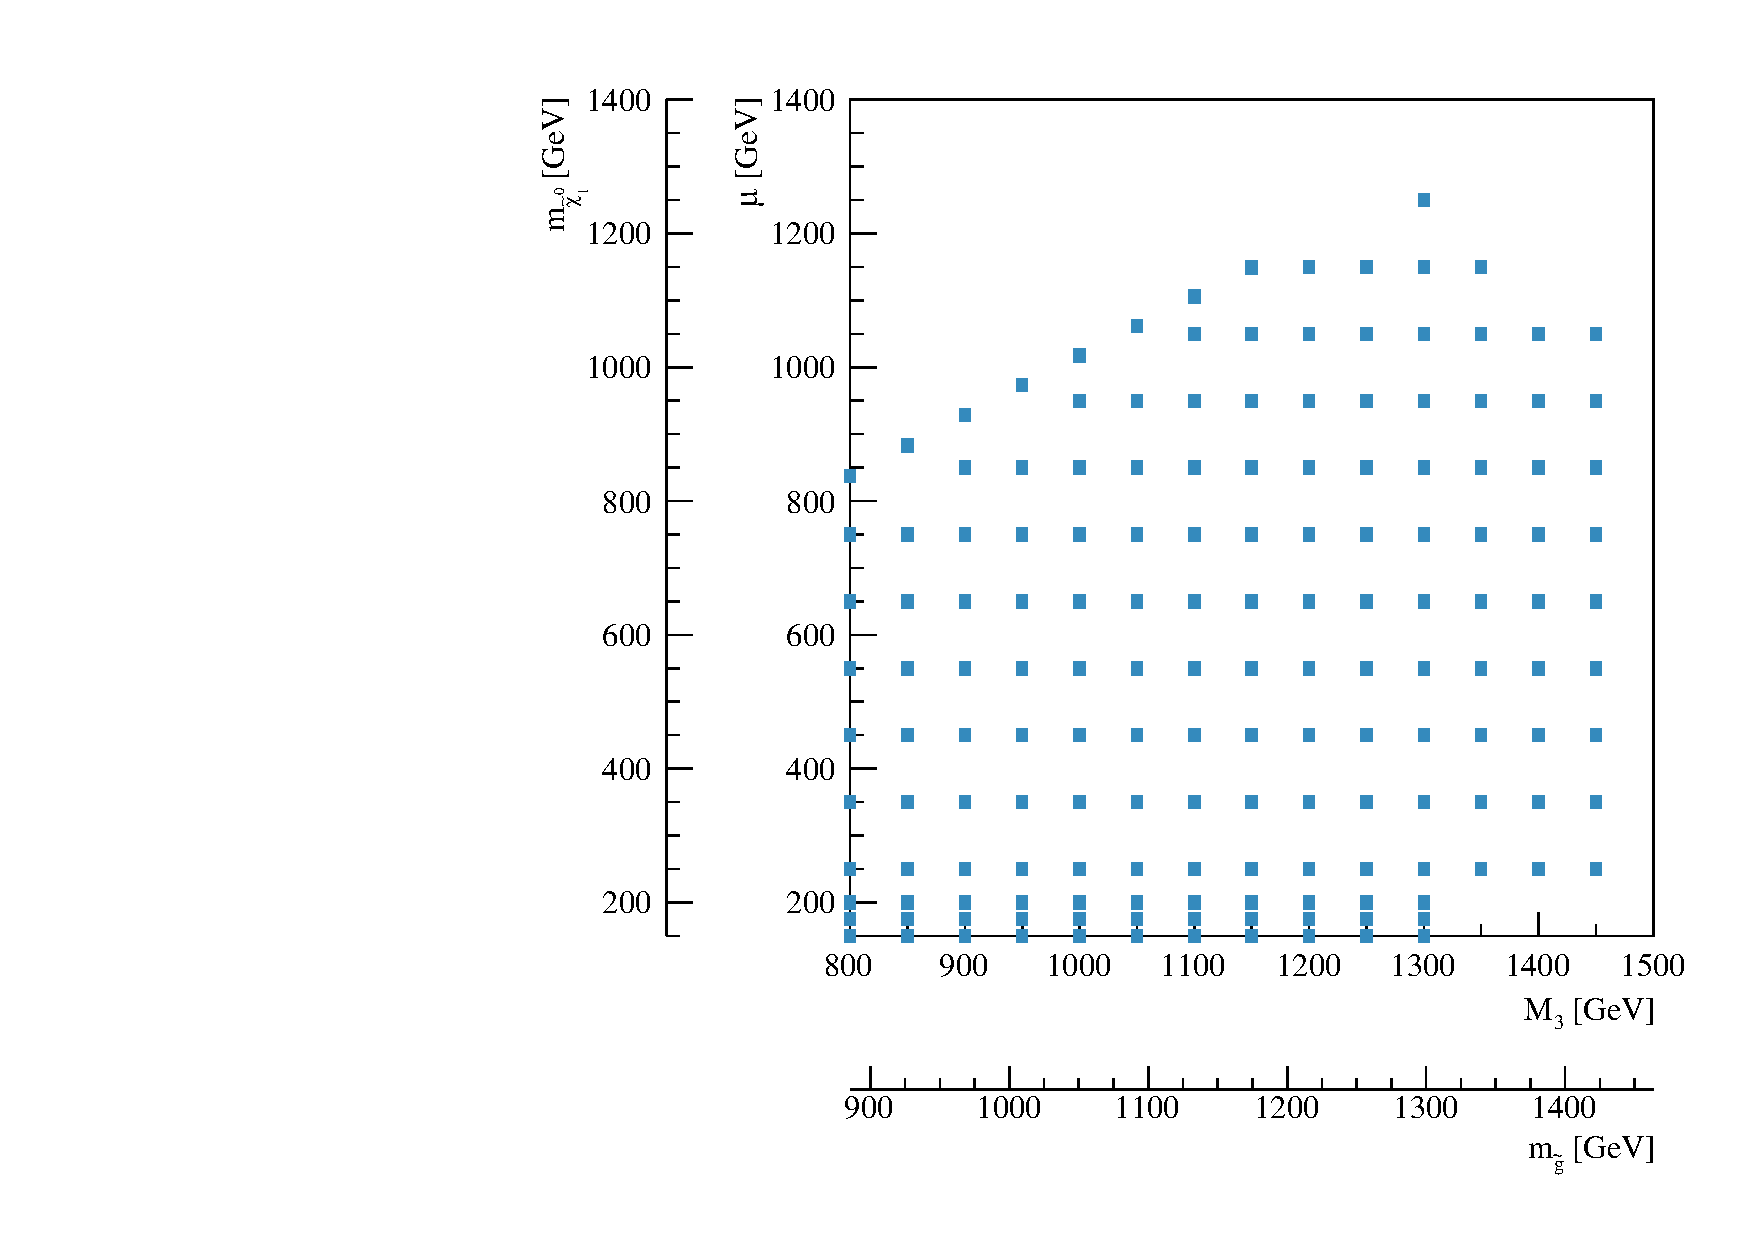
\includegraphics[width=0.5\textwidth]{figures/run1_grid}
  \caption{Update}
  \label{fig:gridpoints}
\end{figure}

%% \M{1} and $\mu$ determine the lightest neutralino mass, and are related in such a way that the branching ratios of the \ninoone\ are approximately constant,
%% resulting in ${\rm BR}(\ninoone \to \gam + \gravino) \approx 50\%$, ${\rm BR}(\ninoone \to Z + \gravino) \approx 49\%$ and ${\rm BR}(\ninoone \to h + \gravino) \approx 1\%$,
%% numbers which vary by $\pm 1\%$ throughout most of the grid ({\fig} \ref{fig:br_n1_x_grav}). For light neutralinos ($<200\gev$) the Higgs production is highly
%% suppressed and ${\rm BR}(\ninoone \to \gam + \gravino)$ starts falling up to 40\%. The value of $\mu$ must also be positive in order to disfavor the branching ratio
%% to the Higgs boson, which would lead to a signature already covered by a dedicated analysis in ATLAS \cite{Aad:2012jva}. Similarly, the branching ratio for
%% ($\ninoone \to \gam + \gravino$) is such that maximizes the single photon final state. At larger values the diphoton topology starts to be favoured, which has been
%% extensively searched for in the past \cite{Aad2012519,Aad:2011kz}. This leaves $M_3$ and $\mu$ as the only two free parameters of the model, spanning the space
%% within $150\gev < m_{\ninoone} < 1250 \gev$ and $800\gev < m_{\gluino} < 1300 \gev$, with $m_{\ninoone} < m_{\gluino}$. The granularity of the simulation in each
%% dimension is shown in {\tab}\ \ref{tab:signal_pars}, with the resulting value for the gluino and neutralino masses.

El espectro completo de masas y los correspondientes decaimientos fueron
calculados a partir de estos parámetros utilizando {\suspect}
(v2.41)\cite{Djouadi2007426}, {\sdecay} (v1.3b)\cite{Muhlleitner:2004mka} y
{\hdecay} (v3.4)\cite{Djouadi:1997yw}, que forman parte del paquete {\susyhit}
(v1.3)\cite{Djouadi:2006bz}.


Algunos ejemplos del espectro de masas puede verse en la
\cref{fig:mass_spectra}, para algunos puntos de la grid.

\begin{figure}[ht!]
   \centering
   \includegraphics[width=0.45\textwidth]{figures/masses_GGM_M3_mu_800_150}
   %%\includegraphics[width=0.45\textwidth]{figures/masses_GGM_M3_mu_1000_750}
   \includegraphics[width=0.45\textwidth]{figures/masses_GGM_M3_mu_1450_1050}

   \caption{Espectro de masas ...}
     %% Solo $M_3$ y $\mu$ son los parámetros libres, en este caso
     %% $(M_3, \mu) = (800~\gev, 250~\gev)$. }
   \label{fig:mass_spectra}
\end{figure}



%%The total decay branching ratios for \gluino-initiated \ninoone\ production are
%% shown in {\fig} \ref{fig:br_gl_n1}, for 2-body\footnote{only effectively, the gluino decays through a virtual
%% quark-squark loop in this case.} and 3-body gluino decays.

Las BR de los neutralinos puede verse en las

\begin{figure}[!ht]
  \centering
  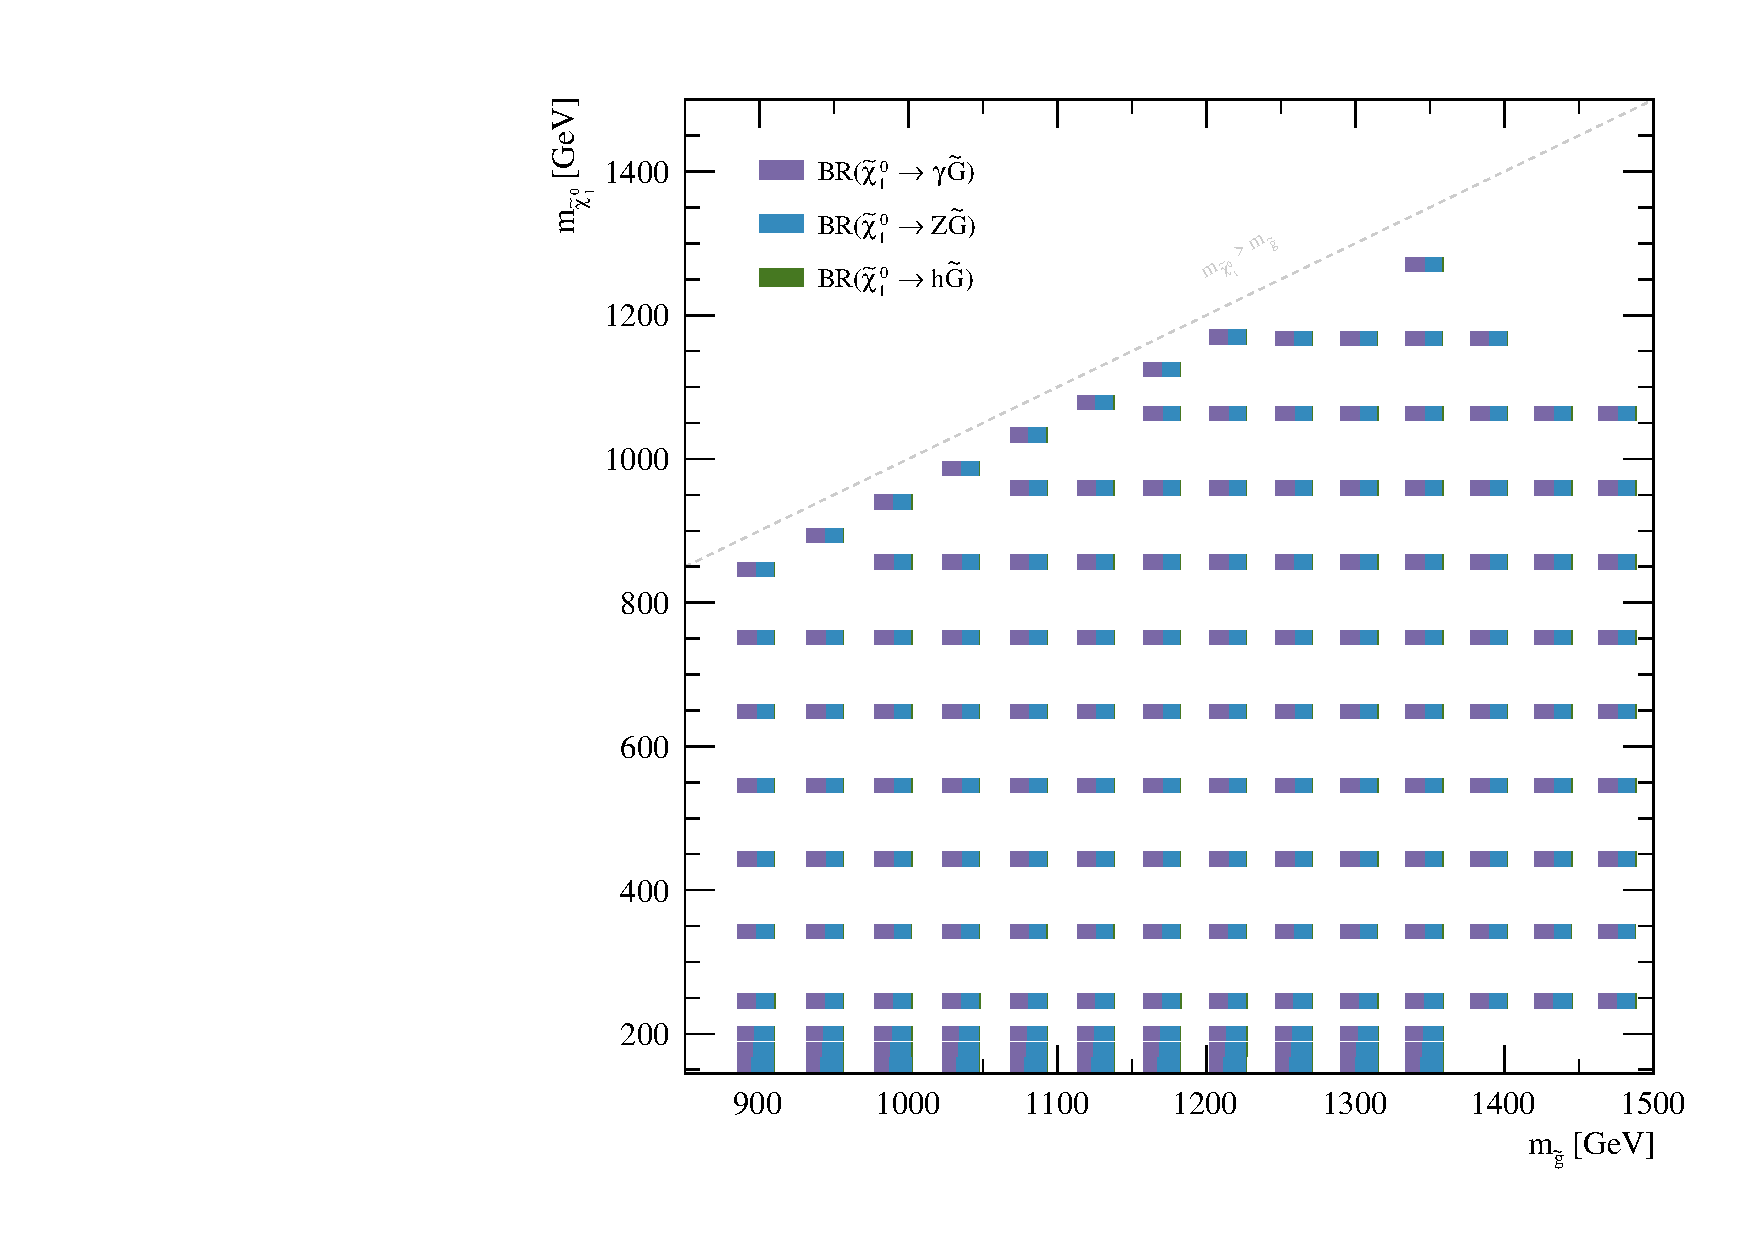
\includegraphics[width=0.3\textwidth]{figures/br_n1_X}
  \includegraphics[width=0.3\textwidth]{figures/br_n2_X}
  \includegraphics[width=0.3\textwidth]{figures/br_n3_X}
\end{figure}


%% -rw-rw-r-- 1 fran fran  17K ago 31 20:38 br_c1_X.pdf
%% -rw-rw-r-- 1 fran fran  21K ago 31 20:38 br_gl_2b_vs_3b.pdf
%% -rw-rw-r-- 1 fran fran  21K ago 31 20:38 br_gl_X_2body.pdf
%% -rw-rw-r-- 1 fran fran  20K ago 31 20:38 br_gl_X_3body.pdf
%% -rw-rw-r-- 1 fran fran  22K ago 31 20:38 br_gl_X.pdf
%% -rw-rw-r-- 1 fran fran  18K ago 31 20:38 br_n1_X.pdf
%% -rw-rw-r-- 1 fran fran  18K ago 31 20:38 br_n2_X.pdf
%% -rw-rw-r-- 1 fran fran  19K ago 31 20:38 br_n3_X.pdf



Se generaron 5000 eventos para cada uno de los 124 puntos de senal, utilizando {\herwigpp} v2.5.2\cite{Bahr:2008pv}
y el conjunto de PDFs CTEQ6L1\cite{Nadolsky:2008zw}. Se aplicó un filtro a nivel generador, que requeria
la presencia de un foton con un {\pt} de al menos 100 \gev, para obtener mas estadistica, especialmente
en los puntos donde el neutralino tiene menor masa. La eficiencia del filtro para todas las muestras
simuladas puede verse en la \cref{tab:signal_filter_eff}.
El pasaje de la senal por el detector ATLAS, fue simulado con la simulacion rapida \textsc{ATLFAST-II}\cite{Richter-Was:683751}.
%% Derived datasets in the {\sc NTUP\_SUSY}
%% format are used throughout this analysis, with the configuration tag p1328.
%% Todas las muestras de señal fueron simuladas con la simulación rápida y perimétrica del detector ATLFAST-II \cite{Richter-Was:683751}.


\subsection{Sección eficaz}

%% La seccion eficaz de produccion y sus incertezas fue calculada usando el paquete SUSYSignalUncertainties \cite{SUSYsigunc}.
%% La seccione eficaz para los procesos que in volucran la produccion de pares de gluinos fueron calculadas a NLO
%% en la constante de acoplamiento fuerte, agregando la \hl{resummation of soft gluon emission at NLO+NLL}\cite{Beenakker:1996ch,Kulesza:2008jb,Kulesza:2009kq,Beenakker:2009ha,Beenakker:2011fu}.
%% La seccion eficas de produccion electrodebil de $\tilde{\chi}\tilde{\chi}$ fue calculada
%% a NLO en la constante de acoplamiento fuerte utilizando {\prospino} \cite{Beenakker:1999xh}.
%% Las secciones eficacez y sus incertezas estan detalladas en la \cref{tab:signal_xs_strong,tab:signal_xs_ewk}
%% y se muestran en las figuras...

En el caso de procesos de producción de pares de gluino o quarks, de los cuales
existe el calculo a NLL, la sección eficaz se toma a NLO en la constante de acoplamiento
fuerte, y se incluye la suma de la emisión de gluones soft con precisión NLL,
realizada utilizando {\nllfast}\cite{Kramer:2012bx,Beenakker:1996ch,Kulesza:2008jb,Kulesza:2009kq,Beenakker:2009ha,Beenakker:2011fu}
.

En el caso de la producción de otro tipo de procesos, como la producción electrodébil, se utiliza
las secciones eficaces calculadas a NLO usando {\prospino}.


\newcommand{\pdfcteqpm}{\ensuremath{\Delta\mathrm{PDF}^{\pm}(\mathrm{CTEQ})}}
\newcommand{\scacteqpm}{\ensuremath{\Delta\mathrm{SCA}^{\pm}(\mathrm{CTEQ})}}

\newcommand{\pdfmstwpm}{\ensuremath{\Delta\mathrm{PDF}^{\pm}(\mathrm{MSTW})}}
\newcommand{\scamstwpm}{\ensuremath{\Delta\mathrm{SCA}^{\pm}(\mathrm{MSTW})}}

\newcommand{\alphap}{\ensuremath{\alpha_s_+}}
\newcommand{\alpham}{\ensuremath{\alpha_s^-}}
\newcommand{\alphapm}{\ensuremath{\alpha_s^{\pm}}}

Las incertezas debidas a la elección de la escala de renormalizacion y
factorizacion como también de la PDF, son obtenidas utilizando {\nllfast} o
calculadas con {\prospino}. En orden de combinar todas estas predicciones y
obtener un incerteza total, se siguen lo mas posible las recomendaciones
PDF4LHC\cite{Botje:2011sn}. Para esto se define la envolvente de las predicciones a la sección eficaz
usando el intervalo a 68\% CL del conjunto de PDFs CTEQ (incluyendo la incerteza en $\alpha_s$ y MSTW,
junto con las variaciones de las escalas. La sección eficaz nominal se obtiene usando el punto medio
de la envolvente y la incerteza como la mitad del ancho de la misma. Matemáticamente
si {\pdfcteqpm} y {\scacteqpm} son las variaciones en $\pm 1\sigma$ de las PDF CTEQ.
Y {\pdfmstwpm} y {\scamstwpm} son las variaciones en $\pm 1\sigma$ en la PDF MSTW.
Y {\alphapm} son las correspondientes incertezas de la constante de acoplamiento fuerte.

\begin{align}
  \Delta\mathrm{CTEQ}^{\pm} &= \sqrt{(\pdfcteqpm)^2 + (\scacteqpm)^2 + (\alphapm)^2} \\
  \Delta\mathrm{MSTW}^{\pm} &= \sqrt{(\pdfmstwpm)^2 + (\scamstwpm)^2}
\end{align}

Los correspondientes extremos por arriba y abajo de la envolvente pueden calcularse a partir de estos:

\begin{align}
  U &= \max(\Delta\mathrm{CTEQ}^\mathrm{nom} + \Delta\mathrm{CTEQ}^{+},\quad \Delta\mathrm{MSTW}^\mathrm{nom} + \Delta\mathrm{MSTW}^{+}) \\
  L &= \min(\Delta\mathrm{CTEQ}^\mathrm{nom} - \Delta\mathrm{CTEQ}^{-},\quad \Delta\mathrm{MSTW}^\mathrm{nom} - \Delta\mathrm{MSTW}^{-})
\end{align}
%
y la seccion eficaz final ($\sigma$) y su incerteza simétrica ($\delta\sigma$) se obtiene como:

\begin{equation}
  \sigma = (U+L)/2,\quad \Delta\sigma = (U-L)/2
\end{equation}

%% \begin{figure}[ht!]
%%    \centering
%%    \includegraphics[width=0.4\textwidth]{figures/n1_gravgam}
%%    \includegraphics[width=0.4\textwidth]{figures/n1_gravz}\\
%%    \includegraphics[width=0.4\textwidth]{figures/n1_gravh}
%%    \caption{Branching ratios of the lightest neutralino (N1) decay. As expected in GGM models,
%%      the gravitino (as LSP) is always produced, in association with either a photon, a Z boson
%%      or a light Higgs boson, depending on the neutralino's nature. The grid parameters in this
%%      analysis have been chosen in order to keep the BR($\ninoone\to\gam\gravino)\sim50$\% across the whole phase space, maximizing the probability of the single photon final state. See text for more details.}
%%    \label{fig:br_n1_x_grav}
%% \end{figure}

%% \begin{table}[ht!]
%%   \centering
%%   \caption{ Model parameters of the GGM signal grid. $M_3$ and $\mu$ are regarded as the free parameters of the model. }
%%   \begin{tabular}{ccc || cccc}
%%     \hline
%%     \hline
%%     $M_3$ [\gev]& $m_{\gluino}$ [\gev]& &  & $\mu$ [\gev]& $M_1$ [\gev]& $m_{\ninoone}$ [\gev] \\
%%     \hline
%%     800  & 885.5   & & & 150  &  300  & 147.0  \tabularnewline
%%     850  & 931.7   & & & 175  &  270  & 168.3  \tabularnewline
%%     900  & 977.6   & & & 200  &  267  & 190.3  \tabularnewline
%%     950  & 1023.1  & & & 250  &  288  & 235.8  \tabularnewline
%%     1000 & 1068.3 & & & 350  &  365  & 332.4  \tabularnewline
%%     1050 & 1113.3 & & & 450  &  456  & 433.2  \tabularnewline
%%     1100 & 1157.9 & & & 550  &  551  & 535.6  \tabularnewline
%%     1150 & 1202.3 & & & 650  &  647  & 638.3  \tabularnewline
%%     1200 & 1246.4 & & & 750  &  745  & 742.0  \tabularnewline
%%     1250 & 1290.3 & & & 838  &  837  & 836.4  \tabularnewline
%%     1300 & 1333.9 & & & 850  &  845  & 846.7  \tabularnewline
%%     1350 & 1377.3 & & & 883  &  882  & 883.7  \tabularnewline
%%     1400 & 1420.5 & & & 928  &  926  & 930.2  \tabularnewline
%%     1450 & 1463.4 & & & 950  &  942  & 949.6  \tabularnewline
%%              &        & & & 973  &  970  & 976.6  \tabularnewline
%%              &        & & & 1017 &  1015 & 1023.4 \tabularnewline
%%              &        & & & 1050 &  1040 & 1053.0 \tabularnewline
%%              &        & & & 1062 &  1058 & 1068.9 \tabularnewline
%%              &        & & & 1106 &  1102 & 1114.8 \tabularnewline
%%              &        & & & 1149 &  1145 & 1160.0 \tabularnewline
%%              &        & & & 1150 &  1140 & 1157.5 \tabularnewline
%%              &        & & & 1250 &  1238 & 1260.6 \tabularnewline
%%     \hline
%%     \hline
%%   \end{tabular}
%%   \label{tab:signal_pars}
%% \end{table}

\begin{table}[ht]
  \centering
  \caption{Sección eficaz a NLO+NLL para la producción de gluinos para los distintos
    puntos de la grid de señal. La ultima columna es la incerteza teórica.}
  \begin{tabular}{cccc}
    \hline
    $M_3$ [\gev] & $m_{\gluino}$ [\gev] & $\sigma$(NLO+NLL) [fb] & Incerteza Total [$\%$]\tabularnewline
    \hline
    800  &  885.5  & 69.05 & 22.5  \\
    850  &  931.7  & 44.92 & 23.8  \\
    900  &  977.6  & 29.73 & 25.2  \\
    950  &  1023.1 & 19.83 & 26.5  \\
    1000 &  1068.3 & 13.41 & 27.7  \\
    1050 &  1113.3 & 9.10 & 29.0  \\
    1100 &  1157.9 & 6.28 & 30.4  \\
    1150 &  1202.3 & 4.32 & 32.0  \\
    1200 &  1246.4 & 3.01 & 33.7  \\
    1250 &  1290.3 & 2.10 & 35.2  \\
    1300 &  1333.9 & 1.48 & 36.7  \\
    1350 &  1377.3 & 1.05 & 38.2  \\
    1400 &  1420.5 & 0.74 & 39.8  \\
    1450 &  1463.4 & 0.53 & 41.5  \\
    \hline
  \end{tabular}
  \label{tab:signal_xs_strong}
\end{table}

\begin{table}[ht]
  \centering
  \caption{Sección eficaz total a NLO para la producción electrodébil de neutralinos y charginos
    para los distintos puntos de la grid de señal. La última columna  es la incerteza
    teórica. Mas detalles se encuentran en la \cref{sec:syst_signal}.}
  \begin{tabular}{cccc}
    \hline
    $\mu$ [\gev] & $m_{\ninoone}$ [\gev] & $\sigma$(NLO) [fb] & Incerteza total [$\%$]\tabularnewline
    \hline
    150   & & 2680 & 6.3  \\
    175   & & 1420 & 6.7  \\
    200   & & 840 & 6.9   \\
    250   & & 280 & 6.4     \\
    350   & & 50 & 7.0    \\
    450   & & 13 & 7.6    \\
    550   & & 4.1 & 8.0  \\
    650   & & 1.4 & 8.5   \\
    750   & & 0.53 & 8.9  \\
    850   & & 0.21 & 9.3  \\
    950   & & 0.0857 & 10.3  \\
    1050  & & 0.0356 & 11.0  \\
    1150  & & 0.0155 & 13.3   \\
    1250  & & 0.00667 & 16.9   \\
    \hline
  \end{tabular}
  \label{tab:signal_xs_ewk}
\end{table}


\begin{table}[ht]
  \centering
  %\small
  \footnotesize
  \caption{Eficiencia del filtro a nivel generador [\%]
    para los puntos de señal simulados.}
  \begin{tabular}{c|ccccccccccccccccc}
    \hline
    \hline
%       &    \multicolumn{11}{c}{Filter efficiency [\%]} \\
%	\hline
     &   \multicolumn{14}{c}{ $M_3$ [\gev] } \\
    $\mu$ [\gev] &  800 & 850 & 900 & 950 & 1000 & 1050 & 1100 &1150 & 1200  & 1250 & 1300 & 1350 & 1400 & 1450 \\
    \hline
    150  &   39.54 &   39.8 &  41.9    &   42.6   &   43.0   &   44.2   &   45.5    &   46.3    &    47.1  &   48.3  &   49.1 &      &      &       \\
    175  &   44.55 &   44.6 &  46.5    &   47.5   &   47.8   &   48.9   &   50.3    &   51.4    &    51.5  &   52.4  &   53.3 &      &      &       \\
    200  &   47.66 &   48.4 &  50.1    &   50.6   &   52.0   &   52.8   &   53.8    &   55.0    &    55.0  &   56.2  &   56.0 &      &      &       \\
    250  &   55.09 &   56.0 &  56.1    &   57.1   &   56.7   &   58.0   &   58.9    &   59.5    &    60.5  &   60.7  &   61.2 & 62.1 & 62.2 &  63.9 \\
    350  &   65.82 &   66.1 &  64.6    &   65.8   &   66.4   &   66.7   &   66.5    &   67.7    &    67.4  &   67.6  &   67.8 & 68.0 & 69.2 &  68.4 \\
    450  &   71.29 &   71.4 &  71.4    &   71.8   &   72.1   &   72.5   &   72.0    &   72.6    &    72.1  &   72.5  &   73.4 & 72.9 & 72.2 &  73.4 \\
    550  &   73.08 &   72.5 &  73.3    &   73.7   &   74.6   &   74.3   &   75.0    &   74.8    &    74.2  &   74.7  &   75.6 & 75.7 & 74.9 &  75.3 \\
    650  &   69.78 &   72.0 &  73.2    &   74.1   &   75.6   &   76.2   &   75.9    &   75.8    &    77.0  &   77.0  &   76.2 & 76.7 & 77.1 &  76.6 \\
    750  &   47.69 &   60.2 &  66.9    &   70.4   &   73.4   &   74.0   &   75.9    &   76.5    &    77.1  &   77.3  &   76.3 & 77.9 & 77.2 &  77.0 \\
    838  &    9.0  &        &          &          &          &          &           &           &          &         &        &      &      &       \\
    883  &         &   9.1  &          &          &          &          &           &           &          &         &        &      &      &       \\
    850  &         &        &  34.2    &   50.7   &   60.1   &   66.4   &   70.4    &   73.5    &    73.6  &   75.4  &   76.6 & 77.1 & 78.2 &  76.8 \\
    928  &         &        &   9.4    &          &          &          &           &           &          &         &        &      &      &       \\
    950  &         &        &          &          &   25.4   &   41.4   &   54.0    &   62.2    &    66.8  &   70.9  &   75.2 & 75.9 & 78.1 &  77.2 \\
    973  &         &        &          &   10.0   &          &          &           &           &          &         &        &      &      &       \\
    1017 &         &        &          &          &   10.3   &          &           &           &          &         &        &      &      &       \\
    1050 &         &        &          &          &          &          &   19.2    &   31.6    &    45.2  &   56.8  &   62.7 & 68.9 & 73.1 &  75.6 \\
    1062 &         &        &          &          &          &   11.1   &           &           &          &         &        &      &      &       \\
    1106 &         &        &          &          &          &          &   11.7    &           &          &         &        &      &      &       \\
    1149 &         &        &          &          &          &          &           &   12.6    &          &         &        &      &      &       \\
    1150 &         &        &          &          &          &          &           &           &    16.1  &   24.9  &   36.9 & 49.0 &      &       \\
    1250 &         &        &          &          &          &          &           &           &          &         &   16.1 &      &      &       \\
    \hline
         \hline
  \end{tabular}
  \label{tab:signal_filter_eff}
\end{table}


%% %\begin{table}[ht]
%% %  \centering
%% %  \small
%% %  \begin{tabular}{|c|c|c|c|c|c|}
%% %    \hline
%% %    \hline
%% %	M3 [\gev] & $\sigma$(NLO+NLL) [\gev] & Uncertainty [$\%$] & k-factor & $m_{\neut}$ [\gev] & Filter efficiency [$\%$] \tabularnewline
%% %    \hline
%% %	\multirow{9}{*}{800} & \multirow{9}{*}{5.96 E-2} & \multirow{9}{*}{26.1} & \multirow{9}{*}{2.84} &  150 &  39.54 \\
%% %    \tiny
%% %	& & & & 175 & 44.55 \\
%% %	& & & & 200 & 47.66 \\
%% %	& & & & 250 & 55.09 \\
%% %	& & & & 350 & 65.82 \\
%% %	& & & & 450 & 71.29 \\
%% %	& & & & 550 & 73.08 \\
%% %	& & & & 650 & 69.78 \\
%% %	& & & & 750 & 47.69 \\
%% %	\hline
%% %	850 & 3.81 E-2 & 27.8 & 2.95 &  150 & 39.8 \tabularnewline
%% %	& & & & 175 & 44.6 \\
%% %	& & & & 200 &  48.4 \\
%% %	& & & & 250 &  56.0 \\
%% %	& & & & 350 &  66.1 \\
%% %	& & & & 450 &  71.4 \\
%% %	& & & & 550 &  72.5 \\
%% %	& & & & 650 &  72.0 \\
%% %	& & & & 750 &  60.2 \\
%% %	\hline
%% %	900 & 2.47 E-2 & 29.5 & 3.07 & 150 & 41.9 \tabularnewline
%% %	& & & & 175 &  46.5 \\
%% %	& & & & 200 &  50.1 \\
%% %	& & & & 250 &  56.1 \\
%% %	& & & & 350 &  64.6 \\
%% %	& & & & 450 &  71.4 \\
%% %	& & & & 550 &  73.3 \\
%% %	& & & & 650 &  73.2 \\
%% %	& & & & 750 &  66.9 \\
%% %	& & & & 850 &  34.2 \\
%% %	\hline
%% %	950 & 1.62 E-2 & 31.4 & 3.19 & 150 & 42.6 \tabularnewline
%% %	& & & & 175 &   47.5 \\
%% %	& & & & 200 &   50.6 \\
%% %	& & & & 250 &   57.1 \\
%% %	& & & & 350 &   65.8 \\
%% %	& & & & 450 &   71.8 \\
%% %	& & & & 550 &   73.7 \\
%% %	& & & & 650 &   74.1 \\
%% %	& & & & 750 &   70.4 \\
%% %	& & & & 850 &   50.7 \\
%% %	\hline
%% %	1000 & 1.08 E-2 & 33.6 & 3.33 & 150 & 43.0 \tabularnewline
%% %	& & & & 175 &   47.8 \\
%% %	& & & & 200 &   52.0 \\
%% %	& & & & 250 &    56.7 \\
%% %	& & & & 350 &    66.4 \\
%% %	& & & & 450 &    72.1 \\
%% %	& & & & 550 &    74.6 \\
%% %	& & & & 650 &    75.6 \\
%% %	& & & & 750 &    73.4 \\
%% %	& & & & 850 &    60.1 \\
%% %	& & & & 950 &    25.4 \\
%% %	\hline
%% %	1050 & 7.19 E-3 & 35.8 & 3.49 & 150 & 44.2 \tabularnewline
%% %	& & & & 175 &   48.9 \\
%% %	& & & & 200 &   52.8 \\
%% %	& & & & 250 &   58.0 \\
%% %	& & & & 350 &   66.7 \\
%% %	& & & & 450 &   72.5  \\
%% %	& & & & 550 &    74.3 \\
%% %	& & & & 650 &    76.2 \\
%% %	& & & & 750 &    74.0 \\
%% %	& & & & 850 &    66.4 \\
%% %	& & & & 950 &    41.4 \\
%% %	\hline
%% %	1100 & 4.87 E-3 & 37.8 & 3.66 & 150 & 45.5 \tabularnewline
%% %	& & & & 175 &   50.3 \\
%% %	& & & & 200 &   53.8 \\
%% %	& & & & 250 &   58.9 \\
%% %	& & & & 350 &   66.5 \\
%% %	& & & & 450 &   72.0 \\
%% %	& & & & 550 &   75.0 \\
%% %	& & & & 650 &   75.9 \\
%% %	& & & & 750 &   75.9 \\
%% %	& & & & 850 &   70.4 \\
%% %	& & & & 950 &   54.0 \\
%% %	& & & & 1050 &  19.2 \\
%% %	\hline
%% %	1150 & 3.29 E-3 & 40.0 & 3.85 &  150 & 46.3 \tabularnewline
%% %	& & & & 175 &   51.4 \\
%% %	& & & & 200 &   55.0 \\
%% %	& & & & 250 &   59.5 \\
%% %	& & & & 350 &   67.7 \\
%% %	& & & & 450 &   72.6 \\
%% %	& & & & 550 &   74.8 \\
%% %	& & & & 650 &   75.8 \\
%% %	& & & & 750 &   76.5 \\
%% %	& & & & 850 &   73.5 \\
%% %	& & & & 950 &   62.2 \\
%% %	& & & & 1050 &  31.6 \\
%% %	\hline
%% %	1200 & 2.24 E-3 & 42.3 & 4.05 &  150 & 47.1 \tabularnewline
%% %	& & & & 175 &   51.5 \\
%% %	& & & & 200 &   55.0 \\
%% %	& & & & 250 &   60.5 \\
%% %	& & & & 350 &   67.4 \\
%% %	& & & & 450 &   72.1 \\
%% %	& & & & 550 &   74.2 \\
%% %	& & & & 650 &   77.0 \\
%% %	& & & & 750 &   77.1 \\
%% %	& & & & 850 &   73.6 \\
%% %	& & & & 950 &   66.8 \\
%% %	& & & & 1050 &  45.2 \\
%% %	& & & & 1150 &  16.1 \\
%% %	\hline
%% %	1250 & 1.55 E-3 & 44.6 & 4.31 & 150 & 48.3 \tabularnewline
%% %	& & & & 175 &   52.4 \\
%% %	& & & & 200 &   56.2 \\
%% %	& & & & 250 &   60.7 \\
%% %	& & & & 350 &   67.6 \\
%% %	& & & & 450 &   72.5 \\
%% %	& & & & 550 &   74.7 \\
%% %	& & & & 650 &   77.0 \\
%% %	& & & & 750 &   77.3 \\
%% %	& & & & 850 &   75.4 \\
%% %	& & & & 950 &   70.9 \\
%% %	& & & & 1050 & 56.8 \\
%% %	& & & & 1150 & 24.9 \\
%% %	\hline
%% %	1300 & 1.07 E-3 & 46.9 & 4.56 & 150 & 49.1 \tabularnewline
%% %	& & & & 175 &   53.3 \\
%% %	& & & & 200 &   56.0 \\
%% %	& & & & 250 &   61.2 \\
%% %	& & & & 350 &   67.8 \\
%% %	& & & & 450 &   73.4 \\
%% %	& & & & 550 &   75.6 \\
%% %	& & & & 650 &   76.2 \\
%% %	& & & & 750 &   76.3 \\
%% %	& & & & 850 &   76.6 \\
%% %	& & & & 950 &   75.2 \\
%% %	& & & & 1050 & 62.7 \\
%% %	& & & & 1150 & 36.9 \\
%% %	& & & & 1250 & 16.1 \\
%% %    \hline
%% %    \hline
%% %  \end{tabular}
%% %  \caption{ The total NLO+NLL cross sections with uncertainties and K factors for GGM  signal points. The last column shows the efficiency of the generator level filter applied, to be considered for the final signal normalization.}
%% %  \label{tab:signal_xs}
%% %\end{table}


%% \begin{figure}[ht!] %  figure placement: here, top, bottom, or page
%%    \centering
%%    \includegraphics[width=0.32\textwidth]{figures/gl_n1g_full}
%%    \includegraphics[width=0.32\textwidth]{figures/gl_n1qq_full}
%%    \includegraphics[width=0.32\textwidth]{figures/gl_n1_full} \\
%%    \includegraphics[width=0.32\textwidth]{figures/gl_n2g_full}
%%    \includegraphics[width=0.32\textwidth]{figures/gl_n2qq_full}
%%    \includegraphics[width=0.32\textwidth]{figures/gl_n2_full} \\
%%    \includegraphics[width=0.32\textwidth]{figures/gl_n3g_full}
%%    \includegraphics[width=0.32\textwidth]{figures/gl_n3qq_full}
%%    \includegraphics[width=0.32\textwidth]{figures/gl_n3_full} \\
%%    \includegraphics[width=0.32\textwidth]{figures/gl_c1qq_full} \\

%%    \caption{Tasas de decaimiento para $\gluino \to \ninoone$,
%%      para todas las posibles cadenas de decaimiento permitidas en la grid
%%      de produccion fuerte. La mayoria de los graficos son la suma
%%      de deciamientos de 2 cuerpos (izquierda) y 3 cuerpos (centro).
%%      Para el decaimiento $\gluino \to \chinopm$), solo el decaimiento de
%%      tres cuerpos es posible.}
%%    \label{fig:br_gl_n1}
%% \end{figure}

%% \clearpage

%% \begin{figure}[ht!]
%%   \centering
%%   \includegraphics[width=0.5\textwidth]{figures/GGM_xs_vs_M3}
%%   \caption{Seccion eficaz de produccion de pares de gluinos como funcion de la masa del gluino, calculada a NLO+NLL con {\nllfast}\hl{fix}.}
%%   \label{fig:signal_xs_vs_M3}
%% \end{figure}

\begin{figure}[htbp]
  \centering
  \subfloat[]{%NLO+NLL cross section $pp \to \gluino\gluino$]{
    \includegraphics[width=0.49\textwidth]{figures/SigXsec_strong}
    \label{fig:signal_xs_strong}
  }
  \subfloat[]{%NLO cross section $pp\to\susy{\chi}\susy{\chi}$]{
    \includegraphics[width= 0.49\textwidth]{figures/SigXsec_ewk}
    \label{fig:signal_xs_ewk}
 }
  \caption{Sección eficaz de producción de pares de gluinos (a)
    y pares de neutralinos/charginos (b).}
  \label{fig:signal_xs}
\end{figure}

\begin{figure}[ht!]
  \centering
  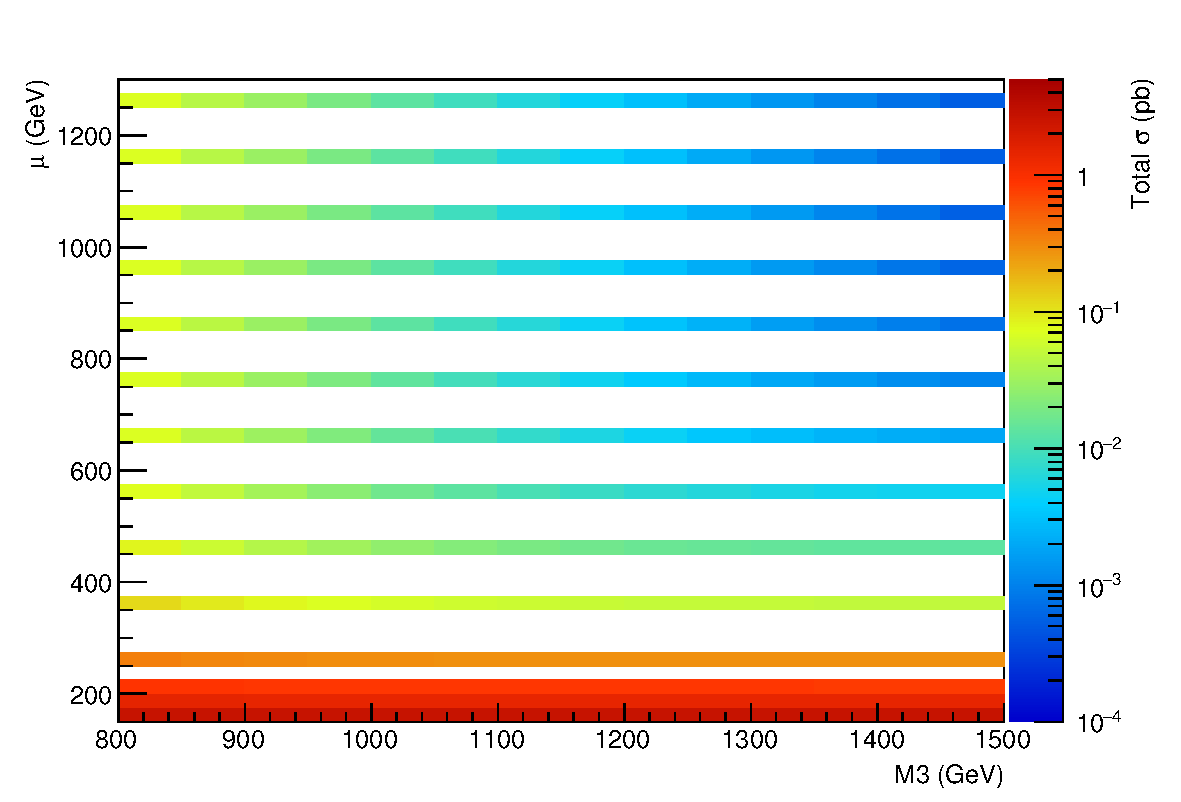
\includegraphics[width=0.49\textwidth]{figures/SigXsec_total}
  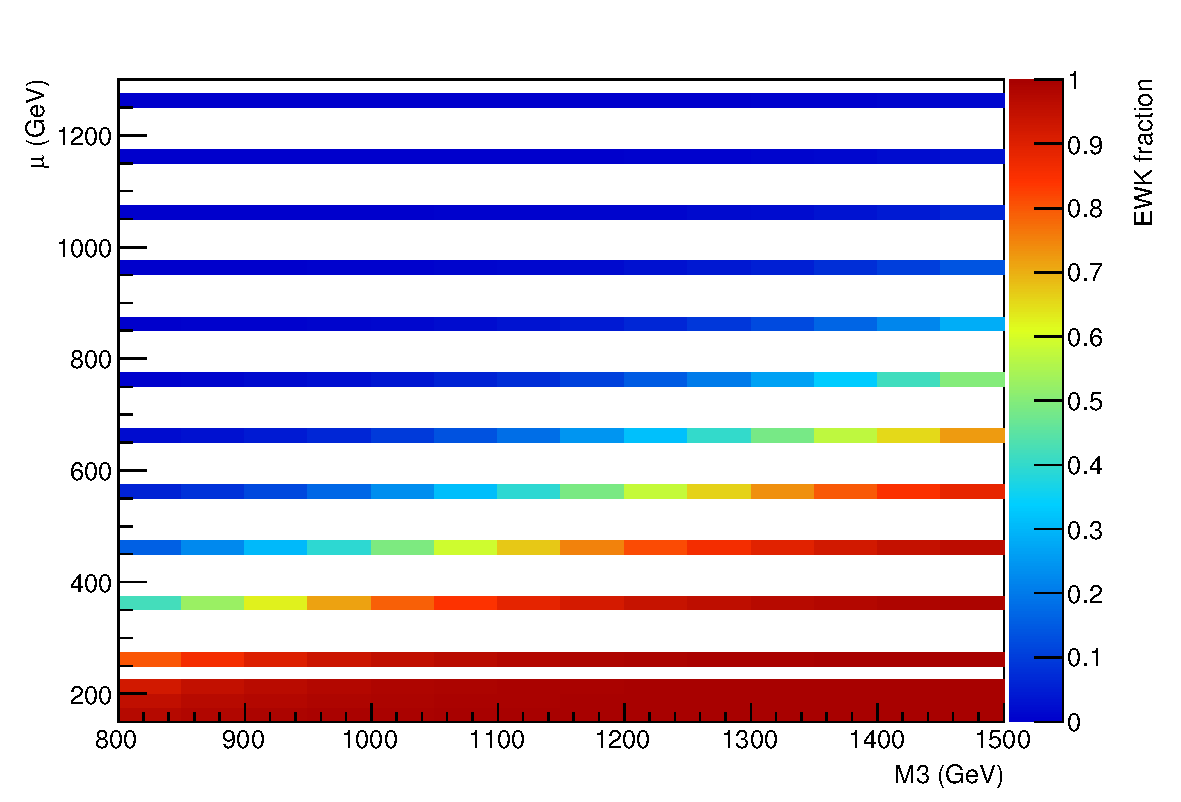
\includegraphics[width=0.49\textwidth]{figures/SigXsec_ewkFrac}
  \caption{Sección eficaz total (izquierda) y fracción relativa
    de producción electrodébil (derecha).}
  \label{fig:signal_xs_total}
\end{figure}


%--------
% Fondos
%--------
\section{Simulación de los fondos del SM}
\label{sec:bkg_samples}

\newcommand{\mccaption}{La sección eficaz a LO para cada modo de decaimiento,
  los factores $k$ (para la normalización NLO) y las eficiencias del filtro
  están detalladas, así como también la luminosidad integrada correspondiente
  a la estadística total de cada muestra.}

Las muestras simuladas con MC utilizadas en este análisis se describen
a continuación. Como se discutirá en la \cref{sec:background_estimation},
la contaminación de fotones mal identificados provenientes de jets y electrones
es estimado con métodos basados en datos. Sin embargo, las muestras MC también
han sido consideradas en estos casos para los estudios de optimización y la
evaluación de las incertezas sistemáticas.

\subsection{$W/Z + \gamma$}

Se espera que la producción de {\wgam} y {\zgam} sea un fondo importante
para esta búsqueda. Ambas muestras fueron generadas usando el generador
de eventos {\sherpa} v1.4.1\cite{SherpaGen}, con hasta 3 partones en el
ME+PS y usando las funciones de densidad partonica CT10.
La combinación de los elementos de matriz con las lluvias partonicas
es realizada de acuerdo a un procedimiento mejorado CKKW\cite{Catani:2001cc,Krauss:2002up}.
Un filtro a nivel generados es aplicado requiriendo al menos un fotón
con $\pt > 80(70) \gev$ en el estado final de las muestras de {\wgam} (\zgam).
Todos los decaimientos leptonicos del bosón $Z$ fueron considerados,
incluyendo el decaimiento invisible $Z\to\nu\nu$.
También se tuvo en cuenta un muestra de $V(\to qq)+\gamma  (V=W,Z/\gamma*)$
debido a que cierta energía faltante real puede  ser producida en el caso
de heavy flavour decays.

\begin{table}[ht!]
  \centering
  \caption{Muestras de W/Z$+\gamma$.
    La sección eficaz a LO se especifica para cada modo de decaimiento,
    al igual que los factores $k$, y las eficiencias del filtro.
    La luminosidad integrada correspondiente a la estadística total
    de cada muestra esta también presente.}
  \begin{tabular}{lccccc}
    \hline
    Proceso & Generador & $\sigma~[pb]$ & $k$ & Eficiencia & $L [fb^{-1}]$ \\
    \hline
    {\wenugam}    & {\sherpa} &  0.7193  &  1.0  &  1.0  &  695.16 \\
    {\wmunugam}   & {\sherpa} &  0.7178  &  1.0  &  1.0  &  696.56 \\
    {\wtaunugam}  & {\sherpa} &  0.7199  &  1.0  &  1.0  &  694.57 \\
    {\zeegam}     & {\sherpa} &  0.1861  &  1.0  &  1.0  &  1069.53 \\
    {\zmumugam}   & {\sherpa} &  0.1858  &  1.0  &  1.0  &  1076.71 \\
    {\ztautaugam} & {\sherpa} &  0.1858  &  1.0  &  1.0  &  1076.19 \\
    {\znunugam}   & {\sherpa} &  0.7625  &  1.0  &  1.0  &  655.74 \\
    {\vqqgam} & {\sherpa}  &  6.756  &  1.0  &  1.0  &  89.0 \\
    %%   \hline
    %%   \multicolumn{5}{l}{Systematics variations} \\
    %%   \hline
    %%    \wenugam (fact. 0.25x) \sherpa (204733) &  0.7193  &  1.0  &  1.0  &  278.05 \\
    %%    \wenugam (fact. 4x) \sherpa (204734) &  0.7193  &  1.0  &  1.0  &  278.05 \\
    %%    \wenugam (renorm. 0.25x) \sherpa (204735) &  0.7193  &  1.0  &  1.0  &  278.05 \\
    %%    \wenugam (renorm. 4x) \sherpa (204736) &  0.7193  &  1.0  &  1.0  &  278.05 \\
    %%    \wenugam (ckkw 15) \sherpa (204731) &  0.7193  &  1.0  &  1.0  &  278.05 \\
    %%    \wenugam (ckkw 30) \sherpa (204732) &  0.7193  &  1.0  &  1.0  &  278.05 \\
    %%    \wmunugam (fact. 0.25x) \sherpa (204739) &  0.7193  &  1.0  &  1.0  &  278.63 \\
    %%    \wmunugam (fact. 4x) \sherpa (204740) &  0.7193  &  1.0  &  1.0  &  278.63 \\
    %%    \wmunugam (renorm. 0.25x) \sherpa (204741) &  0.7193  &  1.0  &  1.0  &  278.63 \\
    %%    \wmunugam (renorm. 4x) \sherpa (204742) &  0.7193  &  1.0  &  1.0  &  278.63 \\
    %%    \wmunugam (ckkw 15) \sherpa (204737) &  0.7193  &  1.0  &  1.0  &  278.63 \\
    %%    \wmunugam (ckkw 30) \sherpa (204738) &  0.7193  &  1.0  &  1.0  &  278.63 \\
    %%    \wtaunugam (fact. 0.25x) \sherpa (204745) &  0.7193  &  1.0  &  1.0  &  277.81 \\
    %%    \wtaunugam (fact. 4x) \sherpa (204746) &  0.7193  &  1.0  &  1.0  &  277.81 \\
    %%    \wtaunugam (renorm. 0.25x) \sherpa (204747) &  0.7193  &  1.0  &  1.0  &  277.81 \\
    %%    \wtaunugam (renorm. 4x) \sherpa (204748) &  0.7193  &  1.0  &  1.0  &  277.81 \\
    %%    \wtaunugam (ckkw 15) \sherpa (204743) &  0.7193  &  1.0  &  1.0  &  277.81 \\
    %%    \wtaunugam (ckkw 30) \sherpa (204744) &  0.7193  &  1.0  &  1.0  &  277.81 \\
    \hline
  \end{tabular}
  \label{tab:bkg_wzgamma_samples}
\end{table}

\subsection{$W/Z$ + jets}
\label{mc_wzjets}

Se espera que la producción de W$^{\pm}$ y bosones $Z$ en asociación con jets
contribuya a esta búsqueda, con los fotones provenientes de electrones y jets
mal identificados. Especialmente para los segundos, esta contaminación no esta
bien descripta por el MC. Por esta razón se utilizan métodos basados en datos
para estimar su contribución en las diferentes regiones de señal y control, como
se describe en el \cref{cap:fondos}. De igual manera varias muestras de MC
fueron consideradas para validar los métodos.

Como se describe en el \cref{cap:seleccion} la selección de señal involucra
muchos jets en el estado final, es importante modelar los estados final multipartonicos
de forma adecuada. Con esto en mente, el generador de eventos {\alpgen} (v 2.14)
fue utilizado, incluyendo los efectos EWK y QCD a LO para los procesos de interacción
fuerte multipartonicos. La producción de jets fue generada for up to five-parton
matrix elements. Este generados fue interfaceado con {\herwig} v6.5.2
para la simulación de las lluvias y los procesos de fragmentación y con {\jimmy}
para la simulación de los eventos subyacentes. Las funciones de densidad partónico
utilizadas fueron las CTEQ6L1. La normalización a la luminosidad integrada acumulada
fue hecha escalenado la sección eficaz mostrada en la \cref{tab:bkg_wzjets_samples}
usando cálculos QCD a NNLO de el programa FEWZ\cite{Anastasiou:2003ds}.
En cada caso los mismos factores de normalización fueron aplicados a los elementos
de matriz de {\alpgen}.

Finalmente, se realiza la remoción de eventos para evitar el conteo doble de eventos
que ya fueron tenidos en cuenta por las muestras de Z$\gamma$ y W$\gamma$.
Para esto, los eventos de $W(Z)+\text{jets}$ con fotones con $\pt > 80(70)\gev$
y $\Delta{\rm R}(e/\mu/\tau/$light-quarks$, \gamma) > 0.1$ fueron removidos
de las muestras.

\begin{table}[ht!]
  \centering
  \caption{Muestras de $W/Z+\text{jets}$. \mccaption.}
  \begin{tabular}{lccccc}
    \hline
    Proceso & Generador & $\sigma [pb]$ & factor-$k$ & Eficiencia & $L [fb^{-1}]$ \\
    \hline
    \zeenj{0} &  \alpgen+\jimmy  & 711.77 & 1.23 & 1 & 7.548 \\
    \zeenj{1} &  \alpgen+\jimmy  & 155.17 & 1.23 & 1 & 6.994 \\
    \zeenj{2} &  \alpgen+\jimmy  & 48.745 & 1.23 & 1 & 6.746 \\
    \zeenj{3} &  \alpgen+\jimmy  & 14.225 & 1.23 & 1 & 6.286 \\
    \zeenj{4} &  \alpgen+\jimmy  & 3.7595 & 1.23 & 1 & 6.487 \\
    \zeenj{5} &  \alpgen+\jimmy  & 1.0945 & 1.23 & 1 & 7.428 \\
    \zmmnj{0} &  \alpgen+\jimmy  & 712.11 & 1.23 & 1 & 7.557 \\
    \zmmnj{1} &  \alpgen+\jimmy  & 154.77 & 1.23 & 1 & 7.011 \\
    \zmmnj{2} &  \alpgen+\jimmy  & 48.912 & 1.23 & 1 & 6.731 \\
    \zmmnj{3} &  \alpgen+\jimmy  & 14.226 & 1.23 & 1 & 6.286 \\
    \zmmnj{4} &  \alpgen+\jimmy  & 3.7838 & 1.23 & 1 & 6.445 \\
    \zmmnj{5} &  \alpgen+\jimmy  & 1.1148 & 1.23 & 1 & 7.292 \\
    \zttnj{0} & \alpgen+\jimmy  & 711.81 & 1.23 & 1 &  7.560 \\
    \zttnj{1} & \alpgen+\jimmy  & 155.13 & 1.23 & 1 &  6.996 \\
    \zttnj{2} & \alpgen+\jimmy  & 48.804 & 1.23 & 1 &  6.746 \\
    \zttnj{3} & \alpgen+\jimmy  & 14.160 & 1.23 & 1 &  6.315 \\
    \zttnj{4} & \alpgen+\jimmy  & 3.7744 & 1.23 & 1 &  6.462 \\
    \zttnj{5} & \alpgen+\jimmy  & 1.1163 & 1.23 & 1 &  7.283 \\
    \hline
    \wenunj{0} & \alpgen+\jimmy  & 8037.10  & 1.186 & 1 & 0.362 \\
    \wenunj{1} & \alpgen+\jimmy  & 1579.20  & 1.186 & 1 & 1.334 \\
    \wenunj{2} & \alpgen+\jimmy  & 477.20   & 1.186 & 1 & 6.661 \\
    \wenunj{3} & \alpgen+\jimmy  & 133.93   & 1.186 & 1 & 6.358 \\
    \wenunj{4} & \alpgen+\jimmy  & 35.62    & 1.186 & 1 & 5.917 \\
    \wenunj{5} & \alpgen+\jimmy  & 10.55    & 1.186 & 1 & 5.592 \\
    \wmnunj{0} & \alpgen+\jimmy  & 8040.00  & 1.186 & 1 & 0.363 \\
    \wmnunj{1} & \alpgen+\jimmy  & 1580.30  & 1.186 & 1 & 1.333 \\
    \wmnunj{2} & \alpgen+\jimmy  & 477.50   & 1.186 & 1 & 6.656 \\
    \wmnunj{3} & \alpgen+\jimmy  & 133.94   & 1.186 & 1 & 6.357 \\
    \wmnunj{4} & \alpgen+\jimmy  & 35.64    & 1.186 & 1 & 6.033 \\
    \wmnunj{5} & \alpgen+\jimmy  & 10.57    & 1.186 & 1 & 1.595 \\
    \wtnunj{0} & \alpgen+\jimmy  & 8035.80  & 1.186 & 1 & 0.353 \\
    \wtnunj{1} & \alpgen+\jimmy  & 1579.80  & 1.186 & 1 & 1.307 \\
    \wtnunj{2} & \alpgen+\jimmy  & 477.55   & 1.186 & 1 & 6.567 \\
    \wtnunj{3} & \alpgen+\jimmy  & 133.79   & 1.186 & 1 & 6.365 \\
    \wtnunj{4} & \alpgen+\jimmy  & 35.58    & 1.186 & 1 & 5.921 \\
    \wtnunj{5} & \alpgen+\jimmy  & 10.54    & 1.186 & 1 & 5.199 \\
    \hline
  \end{tabular}
  \label{tab:bkg_wzjets_samples}
\end{table}


\subsection{Pares de tops ($+\gam$)}
\label{sec:mcttbargam}

Otro fondo importante para este análisis es el {\ttgam}. Esta muestra fue
generada utilizando {\madgraph}\cite{Alwall:2007st} y la PDF CTEQ6L1.
{\pythiasix}\cite{pythia} fue usado para la simulación de las lluvias
partonicas, fragmentación y eventos subyacentes. La radiación de fotones fue
agregadas utilizando {\photos}\cite{photos}, y los decaimientos de los leptones
tau con {\tauola}\cite{tauola}. Se requirió que los fotones a nivel generador
tengan un $\pt > 80 \gev$. Para evitar efectos cinemáticos introducidos por el
filtro, el corte en el {\pt} del fotón en la muestra reconstruida se aumento a
95 {\gev}. Se utilizo un factor-$k$ de $1.9 \pm 0.4$\cite{Melnikov:2011ta, tth}.

Los detalles de la simulación se encuentran en la \cref{tab:bkg_ttbar_samples}.
Se utilizaron además algunas muestras a nivel generador como variaciones para calcular
las incertezas sistemáticas como se explica en la \cref{sec:syst_ttbargamma}.

La producción de {\ttbar}, donde los electrones o los jets son mal identificados
como fotones es una fuente de fondo que vale la pena considerar. Aunque ambas
contaminaciones fueron estimadas a partir de los datos, eventos simulados fueron
utilizados en la etapa de optimización y para chequeos de los métodos. La
muestra MC fue generada utilizando
{\powheg}\cite{Nason:2004rx,Frixione:2007vw,Alioli:2010xd} con la lluvia
partonica y fragmentación hecha por {\pythia}. Para el UE se utilizo Perugia
2011C con el
conjunto de PDFs CTEQ6L1 LO. La radiación de fotones adicional fue agregada con
{\photos}\cite{photos}. Overlap removal is performed to prevent double-counting
the phase-space covered by the {\ttgam} MC sample. Events with truth prompt
photons with $\pt > 95 \gev$ and $\Delta{\rm R}(e/\mu/\tau/g/$light-quarks$,
\gamma) > 0.1$ are removed from the \ttbar\ sample.

\begin{table}[ht!]
  \centering
  \caption{Muestras de {\ttgam}. {\mccaption}}
  \begin{tabular}{lccccc}
    \hline
    Proceso & Generador & $\sigma [pb]$ & factor-$k$ & Eficiencia & $L [fb^{-1}]$ \\
    \hline
    {\ttbar} & \powheg+\pythia & 253.00 & 1 & 0.543 & 580 \\
    \hline
    %    \ttbargam noAllHad \madgraph (164439) & 0.092363 & 1.9 & 1 & 1139.7 \\
    {\ttgam} noAllHad & \madgraph & 0.09873 & 1.9 & 1 & 1066.2 \\
    {\ttgam} AllHad & \madgraph  & 0.068599 & 1.9 & 1 & 1534.5 \\
    \hline
    %% \multicolumn{5}{l}{Variaciones sistematicas} \\
    %% \hline
    %% {\ttgam} noAllHad (scaleUP) & \madgraph & 0.09873 & 1.9 & 1 & 1066.2 \\
    %% {\ttgam} noAllHad (scaleDN) & \madgraph & 0.09873 & 1.9 & 1 & 1066.2 \\
    %% {\ttgam} noAllHad (alpsUP)  & \madgraph & 0.09873 & 1.9 & 1 & 1066.2 \\
    %% {\ttgam} noAllHad (alpsDN)  & \madgraph & 0.09873 & 1.9 & 1 & 1066.2 \\
    %% {\ttgam} noAllHad (moreFSR) & \madgraph & 0.09873 & 1.9 & 1 & 1066.2 \\
    %% {\ttgam} noAllHad (lessFSR) & \madgraph & 0.09873 & 1.9 & 1 & 1066.2 \\
    %% \hline
  \end{tabular}
  \label{tab:bkg_ttbar_samples}
\end{table}

\subsection{Top (+ $\gamma$)}

La producción de un quark top con un fotón asociado fue generado utilizando
\textsc{Whizard} 2.1.1 \cite{whizard, whizard2}, con 4-flavor/5-flavor matching provided
using Hoppet~\cite{hoppet}.

El fotón extra puede estar tanto en la producción del top o en los decaimientos
sucesivos. Sin embargo, la producción y el decaimiento son tratados de forma
separada, por lo que los efectos de interferencia pueden ser ignorados. Para las
lluvias partonicas y la fragmentación fue utilizado {\pythia}\cite{pythia} Y la
radiación de fotones fue agregada con {\photos}\cite{photos}, y los
decaimientos de los leptones tau con {\tauola}\cite{tauola}.

La de producción de tops resulta en un fondo poco importante para este análisis,
aunque de mayor importancia para las regiones control y validación. La producción $Wt$
fue generado utilizando {\powheg}, incluyendo correcciones a NLO en QCD. La lluvia
partónica y la fragmentación fue simulada utilizando {\pythia} con el tune
P2011. Se utilizó el conjunto de PDFs CT10. Las muestras fueron normalizadas con
la sección eficaz calculada en \cite{Kidonakis:2010ux}.
%%Para la produccion en el canal $t$, las muestras MC
%% production, the MC samples with sample ID 110101 were used, with the
%% $W$ boson decaying leptonically. These were generated with
%% \acermc \cite{acer}, with parton showering and fragmentation performed
%% by {\pythia} with the P2011C tune and CTEQ6L1 PDF set.  The samples were
%% scaled to the cross section calculated by \cite{Kidonakis:2011wy}.
%% Single top produced by $s$-channel was not used because it was found
%% to be negligible.
%%Se removieron los  Overlap between the single top and single top $\gamma$ samples has been removed.

\begin{table}[ht!]
  \centering
  \caption{Muestras de quark top y {\tgam}. La sección eficaz a
    NNLO, eficiencia del filtro, y luminosidad integrada correspondiente a la estadística total de cada muestra
    están detalladas.}
  \begin{tabular}{lcccc}
    \hline
    Proceso & Generador & $\sigma [pb]$ & Eficiencia & $L [fb^{-1}]$ \\
    \hline
    t-channel & \acermc   & 28.4 & 1 & 271 \\
    Wt        & \powheg   & 22.4 & 1 & 892 \\
    s-channel & \powheg   & 1.82 & 1 & 3299 \\
    \hline
    \tgam (t-channel) & \wizhard+\pythia   & 0.187298 & 0.121980 & 4810 \\
    \tgam (t-channel) & \wizhard+\pythia   & 0.313866 & 0.012927 & 4930 \\
    \hline
    \twgam (dilep.) & \wizhard+\pythia          & 0.01292  & 0.16437 & 4710 \\
    \twgam (dilep. tDec) & \wizhard+\pythia     & 0.01454  & 0.02875 & 12000 \\
    \twgam (dilep. WDec) & \wizhard+\pythia     & 0.01041  & 0.07549 & 6370 \\
    \twgam (tlepWhad) & \wizhard+\pythia        & 0.02583  & 0.16244 & 4770 \\
    \twgam (tlepWhad tDec) & \wizhard+\pythia   & 0.02908  & 0.02761 & 6230 \\
    \twgam (tlepWhad WDec) & \wizhard+\pythia   & 0.01159  & 0.06471 & 6660 \\
    \twgam (thadWlep) & \wizhard+\pythia      & 0.02582  & 0.16178 & 4790 \\
    \twgam (thadWlep tDec) & \wizhard+\pythia   & 0.02013  & 0.04198 & 5920 \\
    \twgam (thadWlep WDec) & \wizhard+\pythia   & 0.02079  & 0.07574 & 3180 \\
    \hline
  \end{tabular}
  \label{tab:bkg_st_samples}
\end{table}


\subsection{{\gjet} y multijet}

La contaminación QCD es en todos los casos el resultado de eventos patológicos
(jets mal-identificados como fotones, y jets o fotones mal reconstruidos dejando
una alta cantidad de energía faltante). Sin embargo, no se espera que sea un
fondo dominante en el espacio de fase explorado en este análisis. La
contribución de eventos con jets mal identificados como fotones se estima a
partir de los datos en la \cref{sec:jetfakes}.

Las muestras de QCD multijets listadas en \cref{tab:bkg_qcd_samples} fueron
utilizadas para el proceso de optimización y estudios de sensibilidad
preliminares. La producción de fotones prompt fue simulada con {\sherpa}
v1.4.1\cite{SherpaGen}, con hasta cuatro partones en la ME+PS y usando el
conjunto de PDFs CT10. El espectro inclusivo se dividió en secciones del {\pt}
del fotón para optimizar la generación de eventos.

Muestras alternativas fueron utilizadas para la estimación de las incertezas
sistemáticas, generadas con {\pythiaeight} (usando CTEQ6L1) y {\alpgen} v2.14
(con la misma configuración que los eventos de $W/Z +$ jets descriptos en
\cref{mc_wzjets}). Los detalles pueden verse en la \cref{tab:bkg_qcd_samples}.

\begin{table}[ht!]
  \centering
  \caption{Muestras de QCD {\gjet} y multijet utilizadas en este análisis.
    La sección eficaz a LO para cada modo de decaimiento,
    y las eficiencias del filtro están detalladas,
    así como tabine la luminosidad integrada correspondiente a la estadística
    total de cada muestra.}

   \begin{tabular}{lcccc}
    \hline
    Proceso & Generador & $\sigma [pb]$ & Eficiencia & $L [fb^{-1}]$ \\
    \hline
    {\gjet} ($\pt>70\gev$)   & {\sherpa} &    2153.0  &  1.0  &  1.160 \\
    {\gjet} ($\pt>140\gev$)  & {\sherpa} &    137.85  &  1.0  &  10.881 \\
    {\gjet} ($\pt>280\gev$)  & {\sherpa} &     5.963  &  1.0  &  167.657 \\
    {\gjet} ($\pt>500\gev$)  & {\sherpa} &     0.276  &  1.0  &  3617.291 \\
    {\gjet} ($\pt>800\gev$)  & {\sherpa} &    0.0133  &  1.0  &  7492.807 \\
    {\gjet} ($\pt>1000\gev$) & {\sherpa} &   0.00238  &  1.0  &  41980.269 \\
    \hline
    {\gjet} ($\pt>70\gev$)   & {\pythiaeight} &   3425000  &  $0.00057$  &  1535.4  \\
    {\gjet} ($\pt>140\gev$)  & {\pythiaeight} &    122170  &  $0.00097$  &  8449.2 \\
    {\gjet} ($\pt>280\gev$)  & {\pythiaeight} &    3348.7  &  $0.00145$ &  206559.7 \\
    {\gjet} ($\pt>500\gev$)  & {\pythiaeight} &    115.63  &  $0.0018$  &  4789097.0\\
    \hline

    \gjetnj{1} ($\pt>70\gev$)   & {\alpgen}+{\jimmy} &   577.480  &  1.0  &  0.147 \\
    \gjetnj{1} ($\pt>140\gev$)  & {\alpgen}+{\jimmy} &   26.198   &  1.0  &  3.626 \\
    \gjetnj{1} ($\pt>280\gev$)  & {\alpgen}+{\jimmy} &   0.83119  &  1.0  &  30.077 \\
    \gjetnj{1} ($\pt>500\gev$)  & {\alpgen}+{\jimmy} &   0.02914  &  1.0  &  343.159 \\

    % \gjetnj{2} ($\ptgam>35\gev$) \alpgen+\jimmy  ( 156846 ) &  4515.0  &  1.0  &  0.00886 \\
    \gjetnj{2} ($\pt>70\gev$)    & {\alpgen}+{\jimmy} &   571.870  &  1.0  &  0.175 \\
    \gjetnj{2} ($\pt>140\gev$)   & {\alpgen}+{\jimmy} &   38.67100  &  1.0  &  3.879 \\
    \gjetnj{2} ($\pt>280\gev$)   & {\alpgen}+{\jimmy} &   1.6811  &  1.0  &  29.741 \\
    \gjetnj{2} ($\pt>500\gev$)   & {\alpgen}+{\jimmy} &   0.075517  &  1.0  &  264.841 \\

    % \gjetnj{3} ($\ptgam>35\gev$) \alpgen+\jimmy  ( 156851 ) &  1717.0  &  1.0  &  0.00874 \\
    \gjetnj{3} ($\pt>70\gev$)  & {\alpgen}+{\jimmy} &   306.10  &  1.0  &  0.049\\
    \gjetnj{3} ($\pt>140\gev$) & {\alpgen}+{\jimmy} &   28.57  &  1.0  &  5.250 \\
    \gjetnj{3} ($\pt>280\gev$) & {\alpgen}+{\jimmy} &   1.538  &  1.0  &  32.503 \\
    \gjetnj{3} ($\pt>500\gev$) & {\alpgen}+{\jimmy} &   0.07707  &  1.0  &  77.822 \\

    % \gjetnj{4} ($\ptgam>35\gev$) \alpgen+\jimmy  ( 156856 ) &  513.940002  &  1.0  &  0.00778 \\
    \gjetnj{4} ($\pt>70\gev$)    & {\alpgen}+{\jimmy} &   115.850  &  1.0  &  0.216 \\
    \gjetnj{4} ($\pt>140\gev$)   & {\alpgen}+{\jimmy} &   14.216  &  1.0  &  11.951 \\
    \gjetnj{4} ($\pt>280\gev$)   & {\alpgen}+{\jimmy} &   0.9185  &  1.0  &  48.992 \\
    \gjetnj{4} ($\pt>500\gev$)   & {\alpgen}+{\jimmy} &   0.0512  &  1.0  &  156.354 \\

    % \gjetnj{5} ($\ptgam>35\gev$) \alpgen+\jimmy  ( 156861 ) &  163.800003  &  1.0  &  0.0458 \\
    \gjetnj{5} ($\pt>70\gev$)    & {\alpgen}+{\jimmy} &   7.00  &  1.0  &  18.569 \\
    \gjetnj{5} ($\pt>140\gev$)   & {\alpgen}+{\jimmy} &   0.542  &  1.0  &  92.304 \\
    \gjetnj{5} ($\pt>280\gev$)   & {\alpgen}+{\jimmy} &   0.0333  &  1.0  &  450.911 \\
    \gjetnj{5} ($\pt>500\gev$)   & {\alpgen}+{\jimmy} &   44.334  &  1.0  &  0.970 \\

    \hline
    JZ1W ($\pt^{\mathrm{jet}} \in [20, 80] \gev$)     & {\pythia} &   $7.285 \cdot 10^{10}$ &  0.000129 & 0.00016 \\
    JZ2W ($\pt^{\mathrm{jet}} \in [80, 200] \gev$)    & {\pythia} &   $2.634 \cdot 10^{7}$ &  0.003894 & 0.0142 \\
    JZ3W ($\pt^{\mathrm{jet}} \in [200,500] \gev$)    & {\pythia} &   $5.442 \cdot 10^{5}$ &  0.001219 & 2.26 \\
    JZ4W ($\pt^{\mathrm{jet}} \in [500,1000] \gev$)   & {\pythia} &   $0.006445$ &  0.000708 & 328 \\
    JZ5W ($\pt^{\mathrm{jet}} \in [1000,1500] \gev$)  & {\pythia} &   39.74 &  0.002152 & 17400 \\
    JZ6W ($\pt^{\mathrm{jet}} \in [1500,2000] \gev$)  & {\pythia} &   0.4161 &  0.004684 & $7.68 \cdot 10^{5}$ \\
    JZ7W ($\pt^{\mathrm{jet}} > 2000 \gev$)           & {\pythia} &   0.04064 &  0.0146 & $2.52\cdot 10^{6}$ \\
    \hline
  \end{tabular}
  \label{tab:bkg_qcd_samples}
\end{table}

\subsection{Diboson}

Los procesos de diboson (WW, WZ, y ZZ) fueron generados utilizando
{\sherpa} y usando la PDF CT10, con la sección eficaz provista por
MCFM\cite{Campbell:2011bn}. Solo los decaimientos leptonicos para
ambos bosones fueron considerados.

\begin{table}[ht!]
  \centering
  \caption{Muestras de Diboson.
    La sección eficaz a LO para cada modo de decaimiento, los factores $k$
    (para la normalización NLO) y las eficiencias del filtro están detalladas,
    así como también la luminosidad integrada correspondiente a la estadística
    total de cada muestra.}

  \begin{tabular}{lccccc}
    \hline
    Proceso & Generador & $\sigma [pb]$ & factor $k$ & Eficiencia & $L [fb^{-1}]$ \\
    \hline
    %% $WW(2l2\nu)$ \sherpa (126892)  & 5.50 & 1.07 & 1 & 458.9 \\
    %% $WZ(3l)$ \sherpa (126893) & 9.75 & 1.06 & 1 & 261.1 \\
    %% $ZZ(4\ell)$ \sherpa (126894)  & 8.74 & 1.11 & 1  &  185.6 \\
    %% $ZZ(2\ell2\nu)$ \sherpa (126895)  & 0.50 & 1.14 & 1 &  1590.8 \\
    $WW (\ell\ell\nu\nu)$     & {\sherpa}  & 5.296  & 1.06 & 1 & 1400 \\
    $ZZ (\ell\ell\nu\nu)$     & {\sherpa}  & 0.494  & 1.05 & 1 & 1700 \\
    $WZ (\ell\ell\ell\nu)$    & {\sherpa}  & 9.745  & 1.05 & 1 & 260 \\
    $WZ (\ell\nu\nu\nu)$      & {\sherpa}  & 1.406  & 1.05 & 1 & 270 \\
    $ZW (eeqq)$               & {\sherpa}  & 1.465  & 1.05 & 1 & 110 \\
    $ZZ (eeqq)$               & {\sherpa}  & 0.247  & 1    & 1 & 120 \\
    $ZW (\mu\mu qq)$          & {\sherpa}  & 1.463  & 1.05 & 1 & 110 \\
    $ZZ (\mu\mu qq)$          & {\sherpa}  & 0.248  & 1    & 1 & 120 \\
    $ZW (\tau\tau qq)$        & {\sherpa}  & 1.452  & 1.05 & 1 & 120 \\
    $ZZ (\tau\tau qq)$        & {\sherpa}  & 0.242  & 1    & 1 & 120 \\
    $ZW (\nu\nu qq)$          & {\sherpa}  & 2.697  & 1.05 & 1 & 64 \\
    $ZZ (\nu\nu qq)$          & {\sherpa}  & 1.744  & 1    & 1 & 69 \\
    $WW (e\nu qq)$            & {\sherpa}  & 7.285  & 1.06 & 1 & 100 \\
    $WZ (e\nu qq)$            & {\sherpa}  & 1.904  & 1.05 & 1 & 110 \\
    $WW (\mu\nu qq)$          & {\sherpa}  & 7.297  & 1.06 & 1 & 100 \\
    $WZ (\mu\nu qq)$          & {\sherpa}  & 1.906  & 1.05 & 1 & 100 \\
    $WW (\tau\nu qq)$         & {\sherpa}  & 7.274  & 1.06 & 1 & 100 \\
    $WZ (\tau\nu qq)$         & {\sherpa}  & 1.915  & 1.05 & 1 & 100 \\
    \hline
  \end{tabular}
  \label{tab:bkg_diboson_samples}
 \end{table}



%% Referencias
%% \section{Referencias}

%% \begin{itemize}\itemsep0.2cm\parskip0.2cm
%% \item
%% \end{itemize}

%% %% %% MC Event Generators
%% %% @inproceedings{Seymour:2013ega,
%% %%   author         = ``Seymour, Michael H. and Marx, Marilyn'',
%% %%   title          = ``{Monte Carlo Event Generators}'',
%% %%   booktitle      = ``{Proceedings, 69th Scottish Universities Summer School in
%% %%     Physics : LHC Phenomenology (SUSSP69)}'',
%% %%   url            = ``http://inspirehep.net/record/1229804/files/arXiv:1304.6677.pdf'',
%% %%   year           = ``2013'',
%% %%   pages          = ``287-319'',
%% %%   doi            = ``10.1007/978-3-319-05362-2_8'',
%% %%   eprint         = ``1304.6677'',
%% %%   archivePrefix  = ``arXiv'',
%% %%   primaryClass   = ``hep-ph'',
%% %%   reportNumber   = ``MCNET-13-05'',
%% %%   SLACcitation   = ``%%CITATION = ARXIV:1304.6677;%%''
%% %% }
